%Version 3 December 2023
% See section 11 of the User Manual for version history
%
%%%%%%%%%%%%%%%%%%%%%%%%%%%%%%%%%%%%%%%%%%%%%%%%%%%%%%%%%%%%%%%%%%%%%%
%%                                                                 %%
%% Please do not use \input{...} to include other tex files.       %%
%% Submit your LaTeX manuscript as one .tex document.              %%
%%                                                                 %%
%% All additional figures and files should be attached             %%
%% separately and not embedded in the \TeX\ document itself.       %%
%%                                                                 %%
%%%%%%%%%%%%%%%%%%%%%%%%%%%%%%%%%%%%%%%%%%%%%%%%%%%%%%%%%%%%%%%%%%%%%

%%\documentclass[referee,sn-basic]{sn-jnl}% referee option is meant for double line spacing

%%=======================================================%%
%% to print line numbers in the margin use lineno option %%
%%=======================================================%%

%%\documentclass[lineno,sn-basic]{sn-jnl}% Basic Springer Nature Reference Style/Chemistry Reference Style

%%======================================================%%
%% to compile with pdflatex/xelatex use pdflatex option %%
%%======================================================%%

%%\documentclass[pdflatex,sn-basic]{sn-jnl}% Basic Springer Nature Reference Style/Chemistry Reference Style


%%Note: the following reference styles support Namedate and Numbered referencing. By default the style follows the most common style. To switch between the options you can add or remove “Numbered” in the optional parenthesis. 
%%The option is available for: sn-basic.bst, sn-vancouver.bst, sn-chicago.bst%  
 
%%\documentclass[pdflatex,sn-nature]{sn-jnl}% Style for submissions to Nature Portfolio journals
%%\documentclass[pdflatex,sn-basic]{sn-jnl}% Basic Springer Nature Reference Style/Chemistry Reference Style
\documentclass[pdflatex,sn-mathphys-num]{sn-jnl}% Math and Physical Sciences Numbered Reference Style 
%%\documentclass[pdflatex,sn-mathphys-ay]{sn-jnl}% Math and Physical Sciences Author Year Reference Style
%%\documentclass[pdflatex,sn-aps]{sn-jnl}% American Physical Society (APS) Reference Style
%%\documentclass[pdflatex,sn-vancouver,Numbered]{sn-jnl}% Vancouver Reference Style
%%\documentclass[pdflatex,sn-apa]{sn-jnl}% APA Reference Style 
%%\documentclass[pdflatex,sn-chicago]{sn-jnl}% Chicago-based Humanities Reference Style

%%%% Standard Packages
%%<additional latex packages if required can be included here>

\usepackage{graphicx}%
\usepackage{multirow}%
\usepackage{amsmath,amssymb,amsfonts}%
\usepackage{amsthm}%
\usepackage{mathrsfs}%
\usepackage[title]{appendix}%
\usepackage{xcolor}%
\usepackage{color, colortbl}
\usepackage{textcomp}%
\usepackage{manyfoot}%
\usepackage{booktabs}%
\usepackage{algorithm}%
\usepackage{algorithmicx}%
\usepackage{algpseudocode}%
\usepackage{listings}%
\usepackage{comment}
\usepackage{newtxtext,newtxmath}


%% as per the requirement new theorem styles can be included as shown below
\theoremstyle{thmstyleone}%
\newtheorem{theorem}{Theorem}%  meant for continuous numbers
%%\newtheorem{theorem}{Theorem}[section]% meant for sectionwise numbers
%% optional argument [theorem] produces theorem numbering sequence instead of independent numbers for Proposition
\newtheorem{proposition}[theorem]{Proposition}% 
%%\newtheorem{proposition}{Proposition}% to get separate numbers for theorem and proposition etc.

\theoremstyle{thmstyletwo}%
\newtheorem{example}{Example}%
\newtheorem{remark}{Remark}%

\theoremstyle{thmstylethree}%
\newtheorem{definition}{Definition}%

\raggedbottom
%%\unnumbered% uncomment this for unnumbered level heads

\begin{document}
%titulo 75 caracteres contando espacios
\title[Article Title]{Bayesian analysis reveals asymmetry in P2X2 receptor activation}
\author*[1]{\fnm{Luciano} \sur{Moffatt}}\email{lmoffatt@qi.fcen.uba.ar}
\author[2]{\fnm{Gustavo} \sur{Pierdominici-Sottile}}\email{gsottile@unq.edu.ar}
%\equalcont{These authors contributed equally to this work.}

%\author[1,2]{\fnm{Third} \sur{Author}}\email{iiiauthor@gmail.com}
%\equalcont{These authors contributed equally to this work.}

\affil*[1]{\orgdiv{Instituto de Qu\'{i}mica F\'{i}sica de los Materiales, Medio Ambiente y Energ\'{i}a}, \orgname{  Consejo Nacional de Investigaciones Científicas y T\'{e}cnicas}, \orgname{Universidad de Buenos Aires} , \city{Buenos Aires}, \postcode{1428},  \country{Argentina}}

\affil[2]{\orgdiv{Departamento de Ciencia y Tecnolog\'{i}a, 
  Consejo Nacional de Investigaciones Científicas y T\'{e}cnicas} \orgname{Universidad Nacional de Quilmes}, \orgaddress{\street{S\'{a}enz Pe\~{n}a 352}, \city{Bernal}, \postcode{B1876BXD}, \state{Buenos Aires}, \country{Argentina}}}

%\affil[3]{\orgdiv{Department}, \orgname{Organization}, \orgaddress{\street{Street}, \city{City}, \postcode{610101}, \state{State}, \country{Country}}}

\begin{comment}
Voy a tratar de expresar mis ideas de lo que el paper debe decir en comentarios como este. 

Estuve usando mucho chatgpt y un problema que esto genera es que tenes miles de variantes del texto desperdigadas en muchos lugares. 

Por lo tanto voy a tratar de centralizar todos las ideas respecto a lo que debe decir el paper aquí en comentarios. 

nota del 23 de diciembre: 
rehice algunos calculos, 

\end{comment}


\begin{comment}
Cuales son los resultados del paper en orden decreciente de importancia:


Combinando registros de alta resolucion temporal, un modelo cinetico basado en mecanismos conformacionales y un algoritmo bayesiano se obtuvo informacion inesperada respecto a la activacion de receptores purinérgicos. 

Hallazgos mecanisticos: 

1. Hay una asimetria en la activacion de ambas subunidades que forman un mismo sitio de union al agonista. 

1. La union del agonista reduce la barrera energetica para la rotacion de una de las subunidades con las que interactua. 

1. La rotación de la subunidad aumenta la barrera energetica para la union del agonista por el otro sitio de union. 



Presentacion de nuevos algoritmos:

1. una aproximacion a la verosimilitud del promedio temporal de la corriente macroscopica tanto recursiva como no-recursiva. 

2. Un algoritmo de auto-ajuste de los intervalos de temperatura para la intergracion termodinamica que optimiza la convergencia. 

Presentacion de una metodologia para la estimacion efectiva de la evidencia de corrientes macrocópicas. 


Validación de metodologia: 
1. Es posible cuantificar la evidencia de esquemeas cienticos alternativos. Esto permite evaluar hipotesis en forma limpia. 

Cosas que no resuelvo: 
1: deformacion de la señal por parte de los filtros pasabajos. 

Extensiones de este trabajo: 

1. Comparacion de  modelos cineticos con corrientes de canal unico o de pocos canales o de motores moleculares o de mecanismos de difusion. 

2. Analisis del acoplamiento alosterico de la desensitizacion o de otros receptores. 


1. Un novedoso metodo analisis bayesiano compara mecanismos alternativos de activacion de los receptores P2X y demuestra que el mecanismo mas probable dentro de los planteados es un modelo construido a partir de los siguientes supuestos pudimos armar un modelo cinetico que describe la cinetica de activacion de P2X2 

A. Cada subunidad puede rotar sin que las otras necesariamente roten. 
B. La conductancia del canal depende del numero de subunidades rotadas. 
C. La union del agonista es un evento que involucra a tres elementos: el propio agonista y las dos subunidades que conforman el sitio de union. La hipotesis es que la union del agonista se acopla alostericamente con la rotacion de cada subunidad en forma independiente y aditiva. 

Estas tres hipotesis implican un modelo alosterico de dos cambios conformacionales (binding y rotation) y dos acoplamientos (BR y RB: segun sea el binding con la subunidad de la izquierda o derecha). 
Con estos supuestos se encuentra como los cambios conformacionales de una subunidad se propagan por el resto del canal. 
Usando el algoritmo MacroIR pudimos ajustar los parametros de este modelo a una serie experimental de pulsos de concentracion creciente de ATP. 

    

2. A partir de la distribucion a posteriori de los paramteros de acoplamiento cientico de  este modelo cinetico pudimos ver que los acomplamientos alostericos no solo afectan las constantes de equilibrio sino que tambien modulan fuertemente las barreras energeticas. Corroboramos que la union del agonista desplaza el equilibrio hacia la rotacion de la subunidad y viceversa. Corroboramos que este acoplamiento es mas fuerte con una de las subunidades (que a partir de los datos estructurales suponemos que es la unida por el Upper Body) y para sorpresa nuestra encontramos que 
A)la union del agonista ademas reduce la barrera energetica para la rotacion de la subunidad UP (de modo que se incrementan tanto la tasa de rotacion ron como su tasa reversa roff). 
Si la barrera fuera permanentemente baja, el canal responderia igual al agonista sin que se afecte tampoco la conductancia del receptor sin ligando. Solo se verian una mayor frecuencia de rotaciones sin ligando. 
La reduccion del numero de rotaciones tendria valor adaptativo si cada rotacion, cada paso por la barrera energetica conlleve la posibilidad de entrar en un estado inactivo. 


B) la rotacion de la subunidad aumenta la barrera de binding (reduciendo la kon y koff) pero solo de la subunidad LB, la barrera de binding de la otra subunidad no se ve afectada. Esta modulacion explicaria la cooperatividad negativa del binding, donde la afinidad de un sitio disminuye con la union del agonista en el sitio vecino


3. A partir de este modelo pudimos estimar la subconductancia para 1, 2 y 3 subunidades rotadas. Vimos que con dos subunidades se ve una conductancia de entre 1/5 y 1/3 de la conductancia con 3 subunidades. La conductancia de 1 subunidad es marginal. Estos resultados explicaría el hecho que un receptor con solo sitios de union funcionales muestra respuesta al ATP. 


4. La Evidencia de este esquema cinetico es solo inferior a un esquema cinetico convencional con un flip state que bifurca en  dos estados abiertos que confluyen en un cerrado. Los otros modelos alostericos, entre los que se incluye un sincronico, tienen una evidencia inferior. 
Esto muestra todavia hay elementos que nuestro modelo no puede describir adecuadamente, posiblemente relacionados en la desensitizacion. Otra posibilidad es que las rotaciones sigan una cinetica continua. 

5. En este trabajo se ponen en valor varios avances metodologicos: 

A. El mas importante son los cuadrantes del grafico f_on vs f_off que permite separar las situaciones donde cambia la barrera energetica y cuando cambia el salto en energia libre, seprarndo la regulacion cinetica de la termodinamica. Estamos impactados por la simplicidad y profundidad conceptual de esta herramienta, que no entendemos del todo aun. 

B. El desarrollo teorico mas trabajoso y demandante fue el del algoritmo MacroIR. Combinando este algoritmo con un afine-invariante parallel tempering con ajuste dinamico de temperaturas, se lograron hacer analisis cineticos de modelos complejos en situaciones experimentales reales. El costo computacional de este combo esta en el reino de lo posible: ocho nucleos durante dos semanas. Todavia hay mucho por hacer en la optimizacion de este algoritmo. 
Si bien no es necesario calcular la evidencia para obtener la distribucion a posteriori, el metodo de paralel tempering asegura una busqueda exhaustiva en el espacio de parametros, especialmente en situaciones multimodales como todos los modelos medianamente complejos. 


C. Se desarrollo un algoritmo para la construccion automatica de modelos alostericos a partir de indicar un conjunto de cambios conformacionales y sus interacciones. La verificacion de este algoritmo y el desarrollo de una interfaz accesible es un buen material para otro paper. Cuanto incluir de esto en el presente paper es materia a discutir. No es intrumental, deberia ir en otro lado. 

D. Una innovacion interesante es la de incluir ruido rosa en la formulacion de la likelihood. En esta formulacion solo tomamos del mismo la dependencia con la duracion de los intervalos de medicion, no incluimos la correlacion temporal del mismo. La idea es que si existen procesos estocasticos correlacionados (como otros canales en el patch o simplemente procesos que no son descriptos por el modelo plateado) este proceso sea modelado internamente como un ruido rosa. No hicimos un estudio sistematico pero la impresion es que la presencia del ruido rosa ascelera la convergencia de la Evidencia. 





X. Conclusiones metodologicas. El planteo inicial es hipotetico deductivo: a partir de informacion estructural (hipotesis) armamos un modelo cinetico (deduccion)  sin tener en cuenta la informacion cinetica disponible. 
Ahora, la parametrizacion del modelo era amplia y algunos valores de los parametros resultaron inesperados para nosotros, en particular los que determinan que las las barreras energeticas cambiasen. En esto seguimos mas un patron inductivo: a partir de la informacion obtenida formulamos nuevas hipotesis no envisionadas inicialmente. 
La parametrizacion inicial del acoplamiento cinetico alosterico fue extendiendo el concepto de Linear free energy relationship y suponiamos que la pendiente deberia estar entre 0 y 1. No lograrmos buenos ajustes de esta forma y reparametrizamos la relacion extendiendo la parametrizacion de la constante de equilibrio. Esto permitio mejores ajustes, pero no encotrabamos el significado cinetico. Este se hizo claro al graficar las f_on vs f_off y entender   
\end{comment}

\begin{comment}

Este texto surgio de un momento de lucidez


tratemos de ser veridicos

1) pregunta: 
la pregunta original fue como calcular una buena aproximacion a la funcion de likelihood de una macrocorriente. 
La respuesta fue el algoritmo MacroIR. 

La siguiente pregunta fue como saber si este algoritmo da nueva informacion. 

La respuesta fue analizar datos experimentales y comparar esquemas alternativos. 

De ahi surgio otra pregunta: como traducir el conocimiento estructural de la estructura abierta y cerrada a un modelo cinetico?
De alli a una pregunta mas elelemental: como representar en un modelo predictivo la interaccion entre la union al agonista con la apertura del canal? 
La respuesta a esta pregunta esta en los modelos alostericos donde hay un acople de las constantes de equilibrio. 
Ahora la formulacion estandard del alosterismo se restringe a la constante de equilibrio, se plantea entonces la pregunta de como se puede modelar la cinetica del acoplamiento alosterico?
Ahi se extiende la misma idea de los factores alostericos pero a las rates forward y backward (buscar los terminos apropiados). un simple diagrama muestra que en realidad no es que haya alosterismo, sino que el alosterismo es una reparametrizacion de los rates y que se cumple siempre y cuando distingamos los estados como combinacion de los cambios conformacionales. 

Entonces surge la pregunta: como interpreto los factores kineto-alostericos? La primer respuesta a esta pregunta fue usar la analogia con la linear free energy relationship usada para analizar el efecto de mutaciones sobre la cinetica. Pero surgio un problema: se deben permitir exponentes fuera del intervalo 0-1? y ademas fitear en este rango era mas dificil. Se opto por parametrizar contra factores analogos a los del equilibrio tanto sobre los k/r_on como sobre los off. Y esto dio lugar a un resultado que llevo un tiempo interpretar: algunas interacciones asceleraban tanto la kon como la koff y ahi surgio la pregunta: 
que significa la relacion entre los f_kon y f_koff?

Una forma de verlo es a traves de perfiles de energia: el alto de la barrera es proporcional al logaritmo del kon y la diferencia entre kon y koff es proporcional a la constante de equilibrio. 
De esta forma wue  los f_on y f_off sean mayores a uno indican que baja la barrera energetica para la rotacion. 

Finalmente en la discusion surge la pregunta: y qué ventaja tendria bajar la barrera energetica en lugar de tenerla siempre baja (ya que en ambos casos la proporcion de tiempo abierto depende de la keq y no de las f-on y f-off)? 
Una posible respuesta es que el canal podria ser vulnerable durante la rotacion a entrar a un estado irreversible. Y la pregunta aqui es que tipo de configuracion markoviana haria que la entrada a un estado irreversible dependa de la cantidad de cruces? y la respuesta es que la regulacion alosterica seria en la entrada y salida del energetic landscape y no durante la rotacion en si misma. Si la regulacion alosterica afectara a todo el camino, no habria ninguna diferencia en la propension a llegar a un estado irreversible entre una cinetica rapida y una cientica corta. 

Entonces queda la pregunta: y que elementos de la respuesta experimental determinan la caida en la barrera energetica? Respuesta esta en al cinetica del unliganded state: seria relativamente mas lenta que la esperada de no bajar la barrera energetica. 
Ahora todo esto depende de que la corriente en ausencia de ATP se deba exclusivamente a P2X2, las corrientes que no lo son contribuyen al ruido rosa. Un analisis usando MicroIR permitiría distinguir mucho mejor la corriente debida a unliganded P2X2 de otros canales. 

Qué otras preguntas se hicieron?

1) qué es el flip state? la respuesta propuesta en el esquema es que se trata de la rotacion de subunidades.

2) como representar los cambios de conductancia? la respuesta fue suponer que era instantanea y determinada por el numero de subunidades rotadas. No se represento un cambio adicional de gating. como en esquemas anteriores. Esto permitió ajustar la conductancia parcial de 2 subunidades rotadas, una importante prediccion coherente con el hecho de que canales con solo dos sitios de union al atp activos muestran respuesta al ATP. Tambien esto es coherente con observaciones de canal unico donde se obsrvan subconductancias. 

3) es la activacion sincronica o secuencial? Esta disyuntiva se represento en un tabajo anterior, en este trabajo donde se rehacen los modelos sabiendo que el sitio de union es entre subunidades, solo se debe rehacer la alternativa secuencial ya que la sincronica no cambia entre un sitio de union entre subunidades o dentro. La evidencia del modelo sincronico es inferior y multimodal.
\end{comment}


\begin{comment}
comentarios del abstract: 
me llevo el ultimo fin de semana entero pulirlo, siendo asistido por chatgpt. 
Creo que el exceso de chatgpt es muy malo ya que multiplica los textos comos los espejos de Borges. 

Mi sensacion es que pone demasiado enfasis en lo mas espectacular de los resultados (cambios en las barreras) y no en lo mas robusto (que fiteamos el modelo basandonos en consideraciones estructurales).

\end{comment}

\begin{comment}
    Corridas que faltarían hacer, preguntas por contestar: 
1. Cuanta informacion extra se obtiene con MacroIR respecto de MacroINR y cuanto con MacroMR. (scheme_10 vs scheme_9)

2. Concluir las corridas de los esquemas que no confluyeron. 
logL-> 6, 7
logEvi->7,8,9,11

3. tema ruido blanco solo: corrida con scheme_10 solo



3. verificar los requerimientos para el buen comportamiento bayesiano: correr con priors mas amplios en los factores de bayes que me interesen, por ejemplo scheme_10 y 9. 
luego 11 y 6 y 4. 


    
\end{comment}



\begin{comment}
    Table 1 | List of key reporting points for the BARG
Preamble
A. Why Bayesian. If the audience requires it, explain what benefits will be gleaned by a Bayesian analysis (as opposed to a frequentist analysis). [] --> introduction, results or discussion
B. Goals of analysis. Explain the goals of the analysis. This prepares the audience for the type of models to expect and how the results will be described. []-->introduction,methods subsection, results and discussion
Step 1. Explain the model
A. Data variables. Explain the dependent (predicted) variables and independent (predictor) variables[]. -->methods subsection

B. L ikelihood function and parameters. For every model, explain the likelihood function and all the parameters, distinguishing clearly between parameters of primary theoretical interest and
ancillary parameters. If the model is multilevel, be sure that the hierarchical structure is clearly explained, along with any covariance structure if multivariate parameter distributions are
used.  []--> methods subsection
C. Prior distribution. For every model, explain and justify the prior distribution of the parameters in the model.[]-->methods subsection
D. Formal specification. Include a formal specification (mathematical or computer code) of the likelihood and prior, located either in the main text or in in publicly and persistently
accessible online supplementary material. []-->method subsection
E. Prior predictive check. Especially when using informed priors but even with broad priors, it is valuable to report a prior predictive check to demonstrate that the prior really generates simulated data consistent with the assumed prior knowledge. [] -->method subsection (the weight of the prior is clear in some posteriors), the prior is non-informative

Step 2. Report details of the computation --> methods subsection
A. Software. Report the software used, including any specific added packages or plugins. []--> methods subsection
B. MCMC chain convergence. Report evidence that the chains have converged, using a convergence statistic such as PSRF, for every parameter or derived value. [] --->  results  what the fuck is PSRF? do this. 
C. MCMC chain resolution. Report evidence that the chains have high resolution, using the ESS, for every parameter or derived value. [] --> results report ESS
D. If not MCMC. If using some computational procedure other than MCMC, be aware of and report inherently inaccurate approximations, especially for the limits of credible intervals.
Step 3. Describe the posterior distribution
A. Posterior predictive check. Provide a posterior predictive check to show that the model usefully mimics the data. []--> averiguar que es esto 
B. Summarize posterior of variables. For continuous parameters, derived variables and predicted values, report the central tendency and limits of the credible interval. Explicitly state whether you are using density-based values (mode and HDI) or quantile-based values (median and ETI), and state the mass of the credible interval (for example, 95%). -->[] methods subsection 

C. BF and posterior model probabilities. If conducting model comparison or hypothesis testing, report the BF and posterior probabilities of models for a range of prior model probabilities.
[]--> discutir esto en discusion. 

Step 4. Report decisions (if any) and their criteria
A. Why decisions? Explain why the decisions are theoretically meaningful and which decision procedure is being used. Regardless of which decision procedure is used, if it addresses null values, it should be able to accept the null value not only reject it.
[]---> tomamos decisiones? Hipotesis a prueba: 
1. El flip state esta dado por la rotacion de subunidades. 
2. Las subunidades rotan sincronicamente o serialmente. 
3. Las subunidades que comparten un sitio de union responden de manera distinta de acuerdo a como estan unidas al ATP. 
4. El alosterismo no solo se maniesta como alteracion de las constantes de equilibrio sino tambien como modulacion de las barreras energeticas. 
5. La cooperatividad negativa en el binding se debe a la oclusion del sitio de union cuando rota una subunidad impulsada por el otro sitio. 
6. Dos subunidades rotadas alcanzan para generar una corriente medible. 
7. La modulacion de la barrera para rotar permite disminuir la frecuencia de rotaciones del cerrado. 
8. Cada rotacion conlleva una probabilidad de entrar en un estado inactivado, por eso se reduce la frecuencia de las mismas. 

9. La rotacion de una subunidad se ve afectada por la rotacion de la subunidad adyacente. 


B. Loss function. If utilities and a loss function for a decision rule are defined, these should be explained and reported.---> no es aplicable a este trabajo, no tomamos decisiones 


C. ROPE limits. If using a continuous-parameter posterior distribution as the basis for decision, state and justify the limits of the ROPE and the required probability mass.
D. B
 F, decision threshold and model probabilities. If using model comparison or hypothesis testing as the basis for a decision, state and justify the decision threshold for the posterior model
probability, and the minimum prior model probability that would make the posterior model probability exceed the decision threshold.
E. Estimated values too. If deciding about null values, always also report the estimate of the parameter value (central tendency and credible interval).
Step 5. Report sensitivity analysis [] --> subsection in methods
A. For broad priors. If the prior is intended to be vague or only mildly informed so that it has minimal influence on the posterior, show that other vague priors produce similar posterior
results. []--> aca tengo que hacer correr otra cadena. 

B. For informed priors. If the prior is informed by previous research, show what posterior results from a vague prior or from a range of differently informed priors.

C. For default priors. If using a default prior, show the effect of varying its settings. Be sure that the range of default priors constitutes theoretically meaningful priors, and consider whether
they mimic plausible empirically informed priors.
D. B
 Fs and model probabilites. If the analysis involves model comparison or hypothesis testing, then for each prior report not only the BFs but also the posterior model probabilities for a
range of prior model probabilities. [] --> tengo que correr otros esquemas tambien. 

E. Decisions. If making decisions, report whether decisions change under different priors. For BFs, report changes in the minimum prior model probability needed to achieve decisive
posterior model probability.

Step 6. Make it reproducible []--> subsection in methods
A. Software and installation. Explain all the software that is necessary and where to obtain it. If possible, use non-proprietary software. []--> subsection in methods
B. Software version details. The posted script should include detailed information about the software version numbers.
C. S cript and data. Post the complete analysis script (that is, computer code) and data in a stable public repository with persistent URLs, so that anyone can download it and exactly reproduce the analysis. Be sure that it is clear how to navigate the site and find relevant files, for example, with a wiki overview or readme file. If posting data, be sure that it respects privacy and copyright restrictions. If the original data cannot be posted publicly, it may be helpful to post dummy data of the same form so that users can verify the operation of the analysis script.  -->[] aqui con la wiki voy a tener que trabajar, probablmente despues del envio. 

D. R
 eadable for humans. Make the posted script genuinely readable by human beings. Annotate the code with thorough explanatory comments and spatially arrange the code for human
readability.

E. All auxiliary files. Check that all the needed auxiliary files (utility scripts, image files, bibliography files, formatting files and so on) are also posted.
F. Runs as posted. Check that the posted script and accompanying files run as is when downloaded to a different computer. The code should have no lines that load files from personal
computer directories or non-persistent URLs. [] --> modificando los scripts de dirac quizas pueda hacerlo. 

G. MCMC chains for time-intensive runs. For MCMC runs that take a long time to compute, it is helpful to post an MCMC chain so that people can inspect the MCMC chain without having to
wait through an entire run duration. [] --> subirlas a github. 

H. Reproducible MCMC. To make MCMC chains exactly reproducible, the pseudo-random number generators should be explicitly seeded.
\end{comment}





\abstract{
The activation of ligand-gated ion channels is fundamental to cellular signal transduction, impacting diverse processes such as neurotransmission and immune responses. ATP-gated P2X2 receptors, with their structurally simple architecture, provide an accessible model for studying the mechanisms underlying intersubunit allosteric regulation. However, the coordination of ATP-induced conformational transitions in P2X2 remains poorly understood. Here, we demonstrate that the activation kinetics of P2X2 receptors can be accurately reproduced by an asymmetric coupling mechanism, where ATP binding drives the rotation of individual subunits and a saturating increase in conductance as the subunits undergo rotation. Using a novel Bayesian analysis of ultra-short ATP pulse experiments, we demonstrate that ATP binding stabilizes and lowers the energetic barrier for rotation of the left subunit while minimally influencing the right subunit. A second asymmetric coupling explains the negative cooperativity in binding, with ATP binding at one site paradoxically increasing the barrier at the second site. These modulated energy barriers prevent an unliganded rotation that would lead to premature inactivation. Our findings suggest that such tunable activation barriers represent a general strategy for stabilizing ion channels and signaling proteins in dynamic cellular environments. This work provides a mechanistic framework for understanding allosteric regulation in ligand-gated ion channels, with implications for designing therapies targeting P2X receptors in conditions such as chronic pain and inflammation.}




%%================================%%
%% Sample for structured abstract %%
%%================================%%

% \abstract{\textbf{Purpose:} As a guide the abstract should not exceed 200 words. Most journals do not set a hard limit however authors are advised to check the author instructions for the journal they are submitting to.
% 
% \textbf{Methods:} The abstract serves both as a general introduction to the topic and as a brief, non-technical summary of the main results and their implications. The abstract must not include subheadings (unless expressly permitted in the journal's Instructions to Authors), equations or citations. As a guide the abstract should not exceed 200 words. Most journals do not set a hard limit however authors are advised to check the author instructions for the journal they are submitting to.
% 
% \textbf{Results:} The abstract serves both as a general introduction to the topic and as a brief, non-technical summary of the main results and their implications. The abstract must not include subheadings (unless expressly permitted in the journal's Instructions to Authors), equations or citations. As a guide the abstract should not exceed 200 words. Most journals do not set a hard limit however authors are advised to check the author instructions for the journal they are submitting to.
% 
% \textbf{Conclusion:} The abstract serves both as a general introduction to the topic and as a brief, non-technical summary of the main results and their implications. The abstract must not include subheadings (unless expressly permitted in the journal's Instructions to Authors), equations or citations. As a guide the abstract should not exceed 200 words. Most journals do not set a hard limit however authors are advised to check the author instructions for the journal they are submitting to.}

\keywords{Bayesian Analysis, P2X receptors, Cellular Signaling}

\maketitle


\section{Introduction}
\label{sec1}

Ligand-gated ion channels (LGICs) are multimeric membrane proteins that enable ion flux across the cell membrane upon ligand binding \cite{p2x_cuerpo_humano}. These receptors play a crucial role in synaptic transmission, muscle contraction, and numerous physiological processes \cite{p2x_drugs,therapeutic,p2x7_pharmacology}, making them significant targets in neuropharmacology. LGIC families are classified based on their subunit composition and ligand-binding site topology. In pentameric Cys-loop receptors, the binding site is located at the interface between adjacent subunits; in tetrameric glutamate receptors, it resides within individual subunits. P2X receptors, which form trimeric assemblies, share with Cys-loop receptors an inter-subunit binding site arrangement, yet their activation mechanism remains distinct.

P2X receptors are the only LGICs for which high-resolution structures of both open and closed conformations are available \cite{cerrada_p2x,abierta_p2x,estructura_p2x1}. These structures reveal that ATP binding induces a rotational movement in all three subunits, leading to a rearrangement of the transmembrane domains that opens the ion-conducting pore. However, the conformational transitions linking these end states remain unresolved. Understanding these intermediate states is crucial for elucidating the channel activation mechanism and informing the rational design of drugs that modulate P2X receptor function. Structural data suggest that ATP binding stabilizes an asymmetric configuration in which subunits rotate at different rates, raising the question of whether this asymmetry extends to the gating mechanism itself.

Two primary gating models have been proposed for P2X receptor activation: \textit{sequential rotation models}, in which subunits rotate one at a time, and \textit{synchronous models}, where all three subunits transition simultaneously. Within the sequential framework, a key question arises concerning asymmetry: does the first rotating subunit correspond to the one bound by ATP via its Upper Body (UB) or by its Lower Body (LB)? Answering this question is essential for fully understanding P2X receptor activation, with potential implications for the development of allosteric modulators.

In the case of P2X2 receptors, recordings of macroscopic currents in response to ultra-short (0.2 ms) ATP pulses provide valuable insights into the activation process \cite{Moffatt_hume}. Previous models fitted to these data proposed both sequential and synchronous gating schemes. However, these early models incorrectly assumed intrasubunit binding sites, analogous to glutamate receptors, and no formal Bayesian comparison of model evidence had been performed.

To address these limitations, we developed \textit{MacroIR}, a novel likelihood approximation method for macroscopic current analysis. \textit{MacroIR} builds upon our previously introduced \textit{Macroscopic Recursive} (MacroR) algorithm by enabling likelihood calculations for time-averaged current traces over arbitrarily defined intervals. This approach reduces data volume while preserving essential kinetic information, significantly improving computational efficiency. 

Additionally, we introduce two key conceptual advances: \textit{kinetic allosteric coupling} and \textit{conformational models}. Traditional allosteric analysis is often restricted to equilibrium constants, yet receptor activation inherently involves kinetic rate modulation. We extend this framework by defining \textit{kinetic allosteric factors}, which quantify how binding events influence transition rates. Moreover, we define \textit{conformational models} as allosteric models in which all conformational transitions have a well-defined structural correspondence, allowing kinetic parameters to be directly mapped onto molecular mechanisms.

We applied \textit{MacroIR} to analyze our ultrashort ATP pulse recordings of P2X2 receptors. Using an affine-invariant Markov chain Monte Carlo (MCMC) algorithm, we computed posterior distributions and model evidence for alternative kinetic schemes. These schemes were explicitly designed as \textit{conformational models}, incorporating the inter-subunit nature of binding sites and structural differences between the closed and open states, informed by molecular dynamics simulations. Model comparison revealed a striking asymmetry in allosteric coupling: ATP binding reduced the energetic barrier for subunit rotation at the site adjacent to the binding pocket, while subunit rotation increased the energetic barrier for ligand binding at the opposite site. This kinetic asymmetry explains key experimental observations, including the flip state, the sufficiency of two binding sites for channel opening, and the negative cooperativity of agonist binding. Additionally, our analysis showed no evidence for tertiary allosteric coupling, wherein the binding and rotation of one subunit would directly influence the rotation of another.

This study establishes a novel framework for analyzing P2X2 receptor gating by integrating advanced kinetic modeling with the \textit{MacroIR} algorithm. Our findings refine the understanding of P2X receptor activation and introduce a rigorous methodology for bridging kinetic modeling with structural dynamics.

\section{Introduction}
\label{sec1}
\begin{comment}
Leo la introduccion y escribo lo que me genera: 
The key objective of this study is to bridge kinetic and mechanistic insights by addressing a fundamental inverse problem in receptor activation: how can mechanistic models be inferred from kinetic data? While a given mechanism can predict a kinetic course, the reverse—determining the most plausible mechanism from observed kinetics—requires evaluating multiple hypotheses. Here, we propose and rigorously test alternative models, identifying those that best predict the experimental data. This approach necessitates solving two challenges: first, optimizing model parameters to achieve accurate fits to the data; second, comparing alternative models with differing levels of complexity and parameterization.

To address the first challenge, we introduce a novel likelihood approximation for hidden Markov processes, specifically tailored for systems where observable variables are time-averaged. This innovation significantly reduces the data volume required for analysis, enabling efficient parameter fitting even for complex models. For the second challenge, we employ a parallel tempering algorithm, which not only identifies regions of high posterior probability in multi-modal parameter spaces but also calculates the Bayesian evidence, providing a robust basis for model comparison.


\end{comment}


Ligand-gated ion channels (LGICs) are multimeric membrane proteins that allow ions to cross the cell membrane in response to ligand binding \cite{p2x_cuerpo_humano}. These channels play a critical role in synaptic transmission, muscle contraction, and other physiological processes (add them), making them important targets in neuropharmacology \cite{p2x_drugs,therapeutic,p2x7_pharmacology}. LGIC families are classified on the basis of their subunit composition and the location of ligand-binding sites. In pentameric Cys loop receptors, the binding site is located at the interface between adjacent subunits, while in tetrameric glutamate receptors, it is within individual subunits. In trimeric P2X receptors, such as Cys-loop receptors, the binding sites are located between subunits.
\begin{comment}

1er parrafo: Ok

\end{comment}



P2X receptors are the only LGICs for which high-resolution structures of open and closed conformations are available \cite{cerrada_p2x,abierta_p2x}. These structures reveal that ATP binding triggers a rotational movement in all three subunits, leading to separation of the transmembrane domains that form the pore, allowing ions to pass through. However, the intermediate states between these conformations remain unresolved. Understanding these intermediate states is essential for elucidating the mechanism of channel opening, which could inform the design of drugs that modulate the function of the P2X receptor.
\begin{comment}
2do parrafo: falta cita estructure p2x1. 
se podria hacer enfasis en los sitios inter-subunit y quizas en la asimetria del movimiento generado
\end{comment}


Two types of gating models have been proposed for P2X receptor activation: sequential rotation models, where subunits rotate one at a time to gradually open the pore, and synchronous models, where all subunits rotate together in a concerted motion. In sequential models, a key question arises about potential asymmetry: whether one subunit rotates first, specifically the subunit bound to the ATP by the Upper Body (UB) or the one bound by the Lower Body (LB). Addressing this question is essential for understanding the complete activation mechanism of P2X receptors, which could pave the way for innovative pharmacological designs. 

\begin{comment}
3er parrafo: secuencial vs sincronicos
no se los menciona en el abstract, evaluar si mandarlo a discusion
\end{comment}

In the case of P2X2 receptors, recordings of macroscopic currents in response to ultra-short (0.2 ms) ATP pulses provide valuable insight into the channel activation process \cite{Moffatt_hume}. Previous models fitted to these data have proposed sequential and synchronous gating schemes. However, these early models incorrectly assumed intrasubunit binding sites similar to glutamate receptors, and no direct comparison of the evidence for the two gating models has been made. 
\begin{comment}
 4to parrafo: buen hilo con el anterior al tomar lo de secuencial vs sincronico y ahora introducir los inter-subunit
\end{comment}


\section{Introduction}

Macroscopic currents reflect the collective activity of numerous ion channels, and fluctuations in these currents contain valuable kinetic information. To analyze these fluctuations, we developed a novel algorithm, \textit{MacroIR}, which improves upon our previously introduced \textit{Macroscopic Recursive} (MacroR) algorithm by working on currents averaged over arbitrary time intervals. This approach enables data reduction by averaging over exponentially longer intervals after pulse application, significantly decreasing computational load while preserving essential kinetic information. \textit{MacroIR} approximates the likelihood function by calculating the mean state conductance and the variance of the mean over specified time intervals.  

In this work, we introduce two new concepts: \textit{kinetic allosteric coupling} (or simply \textit{kinetic coupling}) and \textit{conformational models}. Traditional allosteric analysis is typically confined to equilibrium constants, but receptor activation also involves kinetic rate modulation. Here, we extend the classical notion of allosteric coupling by defining \textit{kinetic allosteric factors} that directly influence rate constants, providing additional mechanistic insight. Furthermore, we define \textit{conformational models} as those allosteric models in which all conformational transitions and interactions have a clear structural correspondence, allowing a direct connection between kinetic parameters and molecular mechanisms.  

We applied \textit{MacroIR} to our previously published recordings of ultrashort ATP pulses to investigate the gating of the P2X2 receptor. Using an affine-invariant Markov chain Monte Carlo (MCMC) algorithm, we computed posterior distributions and model evidences for alternative kinetic schemes. These schemes were designed as \textit{conformational models}, explicitly incorporating the inter-subunit nature of binding sites and structural differences between the closed and open states of P2X4, informed by molecular dynamics simulations. The comparison of these models revealed a striking asymmetry in allosteric coupling: agonist binding reduced the energetic barrier for subunit rotation at the site adjacent to the binding pocket, while subunit rotation increased the energetic barrier for ligand binding at the opposite site. This kinetic asymmetry explains key phenomena such as the flip state, the sufficiency of two functional binding sites for channel opening, and the negative cooperativity of agonist binding. Additionally, our analysis showed that there is no tertiary allosteric coupling—where binding and rotation of one subunit would influence the rotation of the second subunit.  

Our study provides a novel framework for analyzing P2X2 receptor gating by integrating advanced kinetic modeling with the \textit{MacroIR} algorithm. This approach not only refines our understanding of allosteric mechanisms in ligand-gated ion channels but also establishes a rigorous methodology for bridging kinetic modeling with structural dynamics.  

\begin{comment}
hay que trabajar sobre este parrafo. 
alternativas: 
1) quizas expandir la parte de MCMC y bayesiana a un parrafo
2)quizas expandir el tema de como se generan nuevos modelos alostericos y dar pie a las barreras energeticas
3) definitvamente re-escribir teniendo en cuenta cuales son los resultados del trabajo (ver lista antes del abstract)
\end{comment}


\section{Methods}\label{sec:methods}
We present the experimental data used to evaluate our approach, the kinetic schemes constructed for prediction, the likelihood function quantifying predictive accuracy, and the Evidence determination algorithm for comparing alternative kinetic schemes and inferring posterior parameter distributions.



\subsection{Experimental data: Outside-out Patch recording}

The experimental data used in this study were previously published in The Journal of General Physiology (\cite{Moffatt_hume}) and are reanalyzed here to develop and validate our approach. These data were recorded from macro outside-out patches containing thousands of P2X2 channels, exposed to 0.2-ms pulses of ATP at concentrations of 0.2, 0.5, 1, 2, and 10 mM every 2 minutes, with interspersed 10-ms pulses of 1 mM ATP. The dataset is well-suited for kinetic analysis due to the precise alignment of stimulus timing with channel responses, which were measured directly from the patch \cite{Moffatt_hume}. For further details on the experimental procedure, including the solution compositions, recording conditions, and data acquisition, please refer to the original publication \cite{Moffatt_hume}.
In order to analyze the dataset we did the following: we average at regular 

\subsection{Kinetic schemes under test}
We tested 11 kinetic schemes, including seven previously described by Moffatt and Hume and four new ones developed in this study. The seven established schemes represent progressively complex models of receptor dynamics. Scheme I follows a Monod-Wyman-Changeux (MWC)-like framework with independent binding sites and a single gating transition. Scheme II incorporates an intermediate "flipped" state between the fully bound and open conformations. Scheme III, based on Ding and Sachs (1999), introduces multiple open states converging on a final closed state, while Scheme IV extends this with additional flipping transitions. Schemes V to VII integrate allosteric interactions: Scheme V is an allosteric expansion of the MWC model linking ligand binding to gating, Scheme VI includes a global flipping transition affecting the entire channel, and Scheme VII refines this by allowing flipping to occur independently at each binding site, resulting in a highly interconnected state network. 
At the time this paper was developed, it was not known that the binding site of purinergic receptors was not intra-subunit as in glutamate receptors but inter-subunit as in cys loop receptors. Therefore no though was put into the complexity of the ternary coupling between the binding molecule and both subunits that form the binding site. 
Later the structure of closed and open zP2X4 came out. This solidify the concept of an inter-subunit binding site and a possible mechanism of gating was hinted by the comparison of both structures, where agonist binding induces deformations that facilitate the rotation of the subunits in a concerted way. 
One of the big misteries of the structure was what was the structural correspondence of flipping. Was 
One of the problematic aspects of Schemes VI and VII was that they not only postulated allosteric coupling between binding and flipping and flipping and gating, which make complete sense with flipping being the mechanism that transport the binding energy from the binding site to the gating site, but they postulate, in order to get good fits, direct coupling between binding and gating, which was of much harder interpretation. 
My though was: a different coupling between binding and rotation of the left or right subunit would account for the direct binding-gating mechanism, in the sense that it would explain the variability that as simpler mechanism could not. 
\subsubsection{conductance parametrization}
For one of the top-performing models (Scheme 10), we hypothesized that the current is proportional to the number of rotated subunits. The relationship was modeled by:
\[
i(n) = i_{\text{max}} \cdot \frac{E_n}{E_n + 1}, \quad E_n = E_0 \cdot F_g^n,
\]
where \( E_n \) represents the efficacy of the \( n \)-rotated state. This assumption reduced the number of states by half, significantly enhancing computational feasibility.
A second thought was that we do not have enough computational power to deal with a 48 state model, so we cannot afford a rotation-gating coupling. 
We solve that by assuming that the gating kinetics was too fast and using scheme VI as model, we considered that each rotated subunit contributes to stabilize the open conformation and therefore the mean conductance was a parametrized function of the number of rotated subunits. This trick allow us to halve the number of states, reducing by more than four the computational load. The other advantage of this approach is that it also models the possibility of not having a pore blocking mechanism, that the conductance of the pore is just a non-linear function of the number of rotated subunits. 
In this new schemes we did not talk about flipping but of rotation, because we are mapping conformational changes, not hypothetical ones. Also we  consider allosteric couplings where actual physical contact exist: between  binding and subunit rotation. We consider three couplings: RB (rotation of the right subunit forming the binding site and binding), BR (binding and rotation of the subunit left of the binding site) and RBR (the ternary coupling of binding and rotation of both subunits). 
Four models were built: Scheme VIII, considers only RBR; in Scheme IX and X RBR=1 and they differ in whether RB=BR (IX) or they are independent (X). Scheme XI considers RB, BR and RBR  at the same time. 

\subsubsection{kinetic and equilibrium allosteric factors}
Our previous paper extended the allosteric framework that is usually applied to equilibrium constants to kinetic rates. We added to the usual allosteric factor for the equilibrium constants (which is the same for both coupled conformationa changes), two new allosteric factors: one for each conformational change. 
Lets explain this further. Lets suppose we have two conformational changes g and r. In the absence of interaction, they are described by four independent parameters: $b_{on}$,$b_{off}$,$r_{on}$,$r_{off}$. 
Now suppose we have a BR interaction. Then we will have four new parameters on the activated state: $b^*_{on}$,$b^*_{off}$,$r^*_{on}$,$r^*_{off}$ But, because of microscopic reversibility we know that: 
$$ b_{on} \cdot r^*_{on} \cdot b^*_{off} \cdot r_{off} = r_{on} \cdot b^*_{on} \cdot r^*_{off} \cdot b_{off} $$
or 
$$ \frac {\frac {b_{on}}{b_{off}}}{\frac {b^*_{on}} {b^*_{off}}}     =  \frac {\frac {r_{on}}{r_{off}}}{\frac {r^*_{on}} {r^*_{off}}} =BR_{eq}  $$
Allosterism equivalence is warranted by microscopic reversibility. 
So, we need only two extra parameters to determine the coupled kinetic rates. We choose to define them in terms of the forward rates: 
$$ BR_{b{on}} = \frac{b^*_{on}}{b_{on}}$$
$$ BR_{r{on}} = \frac{r^*_{on}}{r_{on}}$$

For Evidence determination we only used this parameters. However, it was helpful to consider the converse couplings: 
$$ BR_{b{off}} = \frac{b^*_{off}}{b_{off}}$$
$$ BR_{r{off}} = \frac{r^*_{off}}{r_{off}}$$




\subsection{Likelihood function of time averaged macroscopic currents: MacroIR}
In this section we introduce our new algorithm for the determination of the likelihood of time averaged macroscopic currents. This is the heaviest development and it is somewhat complex and it require some Notation.  
As we are introducing a new and we think very usefull technique we will try to be pedagogical, so we will first ilustrate the concepts on the case we have only one channel to build from there the complex case of macrocurrents. Also, we are developing techniques that are also relevant for single channel, so it is worth the space.   

\subsubsection{Notation}
We denote specific channel states using subscripts (e.g., \( i, j \)), while superscripts (e.g., "prior", "post", "obs") are used to indicate the type of probability distribution (e.g., prior, posterior, or observed). For instance, \( p_i^{\text{prior}} \) represents the prior probability of being in state \( i \), and \( p_i^{\text{post}} \) represents the posterior probability after an observation.
\begin{comment}
esta incompleta (me parece)
\end{comment}


\subsubsection{Markov model of single-channel behavior}

Early studies of single-channel recordings revealed that ion channels exhibit stochastic opening and closing at irregular intervals, consistent with the thermal fluctuations that macromolecules experience. Given this stochastic behavior, it is natural to model channel kinetics using a Markov process with a finite set of states \( k \), where each state represents a subset of the channel protein’s conformational landscape. 

A Markov process does not specify the precise conformation of the channel at any given moment; instead, it yields the probability vector \( \boldsymbol{p} \), where each element \( p_i \) represents the likelihood of the channel being in state \( i \). The model assumes a constant transition rate, \( k_{ij} \), for jumps between states \( i \) and \( j \). The time evolution of the probability vector \( \boldsymbol{p}(t) \) is governed by the following first-order differential equation:

\begin{equation}
	\frac{d \boldsymbol{p}}{dt}(t) = \boldsymbol{p}(t) \cdot \boldsymbol{Q}(t),
	\label{eq:master_equation}
\end{equation}

where the off-diagonal elements of the matrix \( \boldsymbol{Q} \) are given by the transition rates \( k_{ij} \). The diagonal elements \( k_{ii} \) are defined to ensure probability conservation:

\begin{align}
	k_{ii} = -\sum_{j, j \neq i} k_{ij}.
	\label{eq:Q_diagonal_element}
\end{align}

This formulation ensures that the total probability remains normalized over time, with the transitions between states governed by the rates encoded in the matrix \( \boldsymbol{Q} \). The Markovian framework thus reduces the complex conformational dynamics of the channel into a tractable probabilistic model, allowing for detailed analysis of the channel gating kinetics.


The integration of Eq.~\ref{eq:master_equation} allows us to determine the time evolution of the probability vector \( \boldsymbol{p}(t) \). This integration yields the following.


\begin{align}
	\boldsymbol{p}(t) &= \boldsymbol{p}(0) \cdot \boldsymbol{P}(t)
	\label{eq:master_equation_solution}
\end{align}
\begin{align}
	\boldsymbol{P} (t) &= \exp(\boldsymbol{Q} \cdot t),
	\label{eq:Transition_Matrix_definition}
\end{align}


where \( \exp(\boldsymbol{Q} \cdot t) \) is the matrix exponential of \( \boldsymbol{Q} \) multiplied by time \( t \). 

In this context, the actual state of the Markov process remains unobservable; what can be directly measured is the current produced by the channel. Each state \( i \) of the channel generates a specific single-channel current, encoded in the current vector \( \boldsymbol{\gamma} \). The observable current at any given time is thus determined by the probability-weighted sum over all states, which can be expressed as:

\begin{equation}
	y^{\text{pred}}(t) = \boldsymbol{p}(t) \cdot \boldsymbol{\gamma}.
	\label{eq:single_channel_prediction}
\end{equation}

This relationship links the hidden Markov states to the measurable macroscopic current, allowing us to infer the channel kinetics from experimental recordings.



\subsubsection{MicroR, Bayesian model for instantaneous measurements of single-channel behavior}

The microscopic recursive term was coined for the exact description of an ensemble of channels, however the equations are the same that for single channels, so we extend the term to cover the classical bayesian analysis fo single channels. 
Consider the scenario where we perform a single "instantaneous" current measurement, denoted as \( y^{\text{obs}} \). Let the initial state probability distribution be given by \( \boldsymbol{p}^{\text{prior}} \). Suppose the instrumental noise associated with each measurement follows a normal distribution with variance \( \epsilon^2 \). Under these conditions, we can derive the likelihood of the measurement and update the posterior probability distribution accordingly.

Using the state current $\gamma_i$, the likelihood of observing the current \( y^{\text{obs}} \) is given by:

\begin{equation}
	\mathcal{L} = P(y^{\text{obs}}) = \sum_i \mathcal{N}(p_i \cdot \gamma_i, \epsilon^2),
	\label{eq:single_channel_likelihood}
\end{equation}

where \( \mathcal{N}(\mu, \sigma^2) \) denotes the normal distribution with mean \( \mu \) and variance \( \sigma^2 \).

The posterior probability distribution, \( \boldsymbol{p}^{\text{post}} \), is then updated using Bayes' rule:

\begin{equation}
	p^{\text{post}}_i = p_i \cdot \frac{\mathcal{N}(p_i \cdot \gamma_i, \epsilon^2)}{P(y^{\text{obs}})},
	\label{eq:single_channel_posterior}
\end{equation}

where \( p^{\text{post}}_i \) denotes the posterior probability of state \( i \) after observing the measurement.

Now, suppose a second measurement is taken after a time interval \( t \). The prior probability distribution at time \( t \), denoted \( \boldsymbol{p}^{\text{prior}}(t) \), is obtained by applying Eq.~\ref{eq:master_equation_solution}:

\begin{align}
	\boldsymbol{p}^{\text{prior}}(t) &= \boldsymbol{p}^{\text{post}}(0) \cdot \boldsymbol{P}(t)
	\label{eq:prior_update}
\end{align}

where \( \boldsymbol{Q} \) is the rate matrix governing the Markov process.

Since the probability of each observation \( {y}_n^{\text{obs}} \) is calculated conditionally on the previous observations \( {y}_1^{\text{obs}}, \dots, {y}_{n-1}^{\text{obs}} \), the cumulative log-likelihood of the entire measurement series can be obtained:

\begin{equation}
	\log \mathcal{L} = \sum_i \log (\mathcal{L}_i),
	\label{eq:total_loglikelihood}
\end{equation}

where \( \mathcal{L}_i \) corresponds to the likelihood of the \( i \)-th measurement.


\subsubsection{MicroIR, the Bayesian Model of Time-Averaged Single-Channel Measurements}

This new algorithm allows to analyze hidden markovian processes where the information we gain from them results from a time-weighed averaged response,as opposed as from an instantaneous observation. It is another solution for the missing events problem, but from a different perspective, one that does not intend to idealize the recording but to directly calculate the likelihood. This would allow to compare the evidence of alternative kinetic models, something that is not straightforward when an idealization step is included.  
We did not actually used this algorithm in this paper, it was necessary conceptual step to present MacroIR. We present it for single channels, but a similar argument can be extended for other single molecule systems, where time averaging is even more compelling (like molecular motors). 
We consider a scenario where, instead of instantaneous measurements, we observe the time-averaged current \( \overline{y_t}^{\text{obs}} \) over a specific interval \( t \). During this time interval, the channel state fluctuates continuously, with each specific trajectory representing a point in an infinite-dimensional space—an unwieldy realm for statistical analysis. However, from a Bayesian perspective, there is only one crucial piece of information: the prior probability distribution at the beginning of each interval. The state probabilities at all subsequent times within the interval can be computed using Eq.~\ref{eq:master_equation_solution}. 

On the other hand, there is only one piece of information that we gain from the interval: the observed average current. Ideally, we would like to obtain the posterior probability at the end of the interval so that it can be used as the prior for the next interval. To correctly compute this posterior distribution, we must account for both the starting and ending states.

Given the prior state probability distribution \( \boldsymbol{p}^{\text{prior}} \) at the start of the interval, we can calculate the joint state probability matrix \( \boldsymbol{\Pi} \), where the elements \( \Pi_{i \rightarrow j} \) represent the probability of starting in state \( i \) and ending in state \( j \):

\begin{equation}
	\Pi_{i \rightarrow j}^{\text{prior}} = p^{\text{prior}}_i \cdot P_{i \rightarrow j}
	\label{eq:joint_state_probability}
\end{equation}

Here, \( P_{i \rightarrow j} \) denotes the probability of transitioning from state \( i \) to state \( j \).

Alternatively, in matrix form:

\begin{equation}
	\boldsymbol{\Pi}^{\text{prior}} = \mathrm{diag}(\boldsymbol{p}^{\text{prior}}) \cdot \mathbf{P}
	\label{eq:joint_state_probability_matrix}
\end{equation}

The probability of an observed average current \( \overline{y}^{\text{obs}} \) result form Eq.~\ref{eq:single_channel_likelihood}:

\begin{equation}
	\mathcal{L}=P(\overline{y}^{\text{obs}}) = \sum_{i, j} \Pi_{i \rightarrow j}^{\text{prior}} \cdot \mathcal{N}\left(\overline{y}^{\text{obs}} - \Pi_{i \rightarrow j}^{\text{prior}} \cdot \overline{\Gamma}_{i \rightarrow j}, \epsilon^2 + \sigma^2_{\overline{\Gamma}_{i \rightarrow j}}\right)
	\label{eq:single_channel_integrated_likelihood}
\end{equation}

where \( \overline{\Gamma}_{i \rightarrow j} \) and \( \sigma^2_{\overline{\Gamma}_{i \rightarrow j}} \) represent the average current and its variance for trajectories starting in state \( i \) and ending in state \( j \), respectively.

The posterior distribution of the joint state probability matrix is updated using Bayes' theorem:

\begin{equation}
	\Pi_{i \rightarrow j}^{\text{post}} = \frac{\Pi_{i \rightarrow j}^{\text{prior}} \cdot \mathcal{N}\left(\overline{y}^{\text{obs}} - \Pi_{i \rightarrow j}^{\text{prior}} \cdot \overline{\Gamma}_{i \rightarrow j}, \epsilon^2 + \sigma^2_{\overline{\Gamma}_{i \rightarrow j}}\right)}{P(\overline{y}^{\text{obs}})}
	\label{eq:single_channel_integrated_posterior}
\end{equation}

The prior state probability distribution for the next interval is then obtained by marginalizing over the initial state \( i \):

\begin{equation}
	p_j^{\text{prior}}(t_{n+1}) = \sum_i \Pi_{i \rightarrow j}^{\text{post}}(t_n)
	\label{eq:single_channel_integrated_next_prior}
\end{equation}

Since the probability of each observation \( \overline{y}_n^{\text{obs}} \) is calculated conditionally on the previous observations \( \overline{y}_1^{\text{obs}}, \dots, \overline{y}_{n-1}^{\text{obs}} \), the cumulative log-likelihood of the entire measurement series can be updated using Eq. \ref{eq:total_loglikelihood}:

\begin{equation}
	\log \mathcal{L}(\overline{y}_1^{\text{obs}}, \dots, \overline{y}_{n+1}^{\text{obs}}) = \log \mathcal{L}(\overline{y}_1^{\text{obs}}, \dots, \overline{y}_n^{\text{obs}}) + \log P(\overline{y}_{n+1}^{\text{obs}})
	\label{eq:single_channel_integrated_total_likelihood}
\end{equation}

While the exact distribution of the mean current is not strictly normal, we approximate it as such, assuming that instrumental noise dominates over gating noise.

\subsubsection{Calculation of the Average Current Conditional on Starting and Ending States}

We calculate the average current \( \overline{\Gamma}_{i \rightarrow j} \) and its variance \( \sigma^2_{\overline{\Gamma}_{i \rightarrow j}} \) for transitions from state \( i \) to state \( j \) during a measurement interval \( t \).

The average current \( \overline{\Gamma}_{i \rightarrow j} \) is computed as the time-weighted average of the current in each state, weighted by the probability of being in that state during the interval:

\begin{equation}
	\overline{\Gamma}_{i \rightarrow j} = \frac{1}{t \cdot P_{i \rightarrow j}} \int_0^t \sum_k P_{i \rightarrow k}(\tau) \, \gamma_k \, P_{k \rightarrow j}(t - \tau) \, d\tau
	\label{eq:gamma_ij_integral}
\end{equation}

Here, \( P_{i \rightarrow j} \) is the probability of transitioning from state \( i \) to state \( j \) within time \( t \), \( P_{i \rightarrow k}(\tau) \) denotes the probability of transitioning from state \( i \) to state \( k \) at time \( \tau \), and \( \gamma_k \) is the current associated with state \( k \).

To efficiently evaluate this integral, we use a spectral form of the matrix exponential, yielding a closed-form expression:

\begin{equation}
	\overline{\Gamma}_{i \rightarrow j} = \frac{1}{P_{i \rightarrow j}} \sum_{k, n_1, n_2} V_{i n_1} \cdot V^{-1}_{n_1 k} \cdot \gamma_k \cdot V_{k n_2} \cdot V^{-1}_{n_2 j} \cdot E_2(\lambda_{n_1} \cdot t, \lambda_{n_2} \cdot t)
	\label{eq:gamma_ij_formula}
\end{equation}

where:
- \( \mathbf{V} \) and \( \mathbf{V}^{-1} \) are the matrices of eigenvectors of the rate matrix \( \mathbf{Q} \) and its inverse, respectively.
- \( \boldsymbol{\lambda} \) is the vector of eigenvalues of \( \mathbf{Q} \).
- The function \( E_2(x, y) \) is defined as:

\begin{equation}
	E_2(x, y) = 
	\begin{cases}
		\frac{\exp(x) - \exp(y)}{x - y}, & \text{if } x \neq y \\
		\exp(x), & \text{if } x = y
	\end{cases}
    \label{eq:E_2}
\end{equation}


\subsubsection{Calculation of the Variance of the Average Current Conditional on Starting and Ending States}

The variance of the average current, conditional on starting in state \(i\) and ending in state \(j\), is defined as the difference between the expected square of the average current and the square of the expected current:

\begin{equation}
	\sigma^2 \overline{\Gamma}_{i \rightarrow j}=\text{Var}(\overline{\Gamma}_{i \rightarrow j}) = E(\overline{\Gamma}_{i \rightarrow j}^2) - P_{i \rightarrow j} \cdot \left( E(\overline{\Gamma}_{i \rightarrow j}) \right)^2
    \label{eq:sigma_gamma_expression}
\end{equation}

where \( E(\overline{\Gamma}_{i \rightarrow j}^2) \) is the expected square of the average current, and \( E(\overline{\Gamma}_{i \rightarrow j}) \) is the expected average current.


To calculate the expected square of the average current, we consider the time-weighted average of the product of the currents at each pair of time points within the interval. This involves summing over all possible intermediate states \(k_1\) and \(k_2\) for the first and second currents, respectively. Specifically, we integrate over the full time interval, accounting for all combinations of transition probabilities at each time point:

\begin{equation}
	E(\overline{\Gamma}_{i \rightarrow j}^2) = \frac{1}{t^2 P_{i \rightarrow j}} \int_0^t \int_0^{t-\tau_1} \sum_{k_1, k_2} P_{i \rightarrow k_1}(\tau_1) \gamma_{k_1} P_{k_1 \rightarrow k_2}(\tau_2) \gamma_{k_2} P_{k_2 \rightarrow j}(t-\tau_1-\tau_2) d\tau_1 d\tau_2
    \label{eq:sqr_gamma_integral}
\end{equation}

Here, \(P_{i \rightarrow k_1}(\tau_1)\) and \(P_{k_1 \rightarrow k_2}(\tau_2)\) represent the transition probabilities between states over the respective time intervals \(\tau_1\) and \(\tau_2\), and \(\gamma_{k_1}\) and \(\gamma_{k_2}\) denote the currents in those states.


By utilizing the spectral decomposition of the transition rate matrix, we can obtain a closed-form expression for the expected square of the average current. This allows us to express the quantity in terms of matrix products and the eigenvalues of the transition rate matrix, as shown below:

\begin{equation}
	E(\overline{\Gamma}_{i \rightarrow j}^2) = \frac{1}{P_{i \rightarrow j}} \sum_{k_1, k_2, n_1, n_2, n_3} V_{i n_1} \cdot V^{-1}_{n_1 k_1} \cdot \gamma_{k_1} \cdot V_{k_1 n_2} \cdot V^{-1}_{n_2 k_2} \cdot \gamma_{k_2} \cdot V_{k_2 n_3} \cdot V^{-1}_{n_3 j} E_3(\lambda_{n_1} \cdot t, \lambda_{n_2} \cdot t, \lambda_{n_3} \cdot t)
    \label{eq:sqr_gamma_formula}
\end{equation}

Here, \(E_3\) is a function that acts on the eigenvalues of the transition rate matrix, and is defined as follows:

\begin{equation}
	E_3(x,y,z)= 
	\begin{cases}
		E_{111}(x,y,z) & x\neq y, y\neq z, z\neq x \\
		E_{12}(x,y) & x\neq y, x\neq z, y = z \\
		E_{12}(y,z) & y\neq z, y\neq x, z = x \\
		E_{12}(z,x) & z\neq x, z\neq y, x = y \\
		\frac{1}{2} \cdot \exp(x) & x=y=z
	\end{cases}
	\label{eq:E_3}
\end{equation}

The function \(E_{12}(x, y)\) is defined as:

\begin{equation}
	E_{12}(x,y) = E_{1,11}(x, y, y) + \frac{\exp(y)}{y - x} \cdot \left(\frac{y - x - 1}{y - x}\right)
	\label{eq:E_12}
\end{equation}

Finally, \(E_{1,11}(x, y, z)\) is given by:

\begin{equation}
	E_{1,11}(x, y, z) = \frac{\exp(x)}{(x - y) \cdot (x - z)}
	\label{eq:E_1_11}
\end{equation}

These expressions allow us to compute the expected square of the average current in a system where the transitions between states are governed by a Markov process with a known transition rate matrix.






\subsubsection{From Single-Channel Analysis to Ensemble Channel Analysis}

When the only information available about an ensemble of ion channels is the state probability vector—which specifies the likelihood of each individual channel being in a particular state—a multinomial distribution describes the probability of observing each possible distinct state count vector. However, once we gain additional information by measuring the total current produced by the ensemble, we can update the posterior distribution of the ensemble state. This updated distribution not only deviates from a multinomial form but also exhibits inverse correlations between states that generate the same current. Although individual channels remain independent, the information we obtain about the ensemble as a whole introduces correlations, reminiscent of quantum entanglement. Thus, we require a method to characterize the posterior probability distribution of the ensemble state that adequately captures these induced correlations.

A precise yet computationally intensive approach involves constructing a vector—referred to as the \textit{ensemble state vector}—that encompasses all possible combinations of state counts and applying Bayes' rule to each entry individually. This method, which I term the \textit{Microscopic Recursive Algorithm}, was detailed in a previous publication (Moffatt, 2007). However, this approach quickly becomes computationally prohibitive as the system size increases.

A more efficient alternative approximates the ensemble state distribution using a multivariate normal distribution of the state count vector. The covariance matrix serves as a first-order approximation to account for the observation-induced correlations between states. This constitutes the \textit{Macroscopic Approach}, significantly simplifying the representation of the ensemble's state distribution.

\subsubsection{MacroR, Bayesian Framework for Instantaneous Measurements of Channel Ensembles}

In the \textit{MacroR algorithm}, we treat measurements as instantaneous and focus solely on the ensemble's instantaneous state. This framework leverages both the mean probability vector and the covariance matrix of the probability state, capturing the ensemble's key statistical properties at any given moment. The same results can be obtained from a Kalman filter. 

After integrating the multivariate Gaussian, the likelihood of observing an instantaneous current \( y^{\text{obs}} \) can be obtained:

\begin{equation}
	\mathcal{L} = \mathcal{N} \left( y^{\text{obs}} - y^{\text{pred}}, \sigma^2_{y^{\text{pred}}} \right)
	\label{eq:macro_likelihood}
\end{equation}

where \( y^{\text{pred}} \), the prediction of the kinetic model for the subsequent observation, is given by:

\begin{equation}
	y^{\text{pred}} = N_{\text{ch}} \cdot \boldsymbol{\mu}^{\text{prior}} \cdot \boldsymbol{\gamma}
	\label{eq:macro_predicted_y}
\end{equation}

Here, \( \sigma^2_{y^{\text{pred}}} \), the variance of this prediction, which is related to what is usually called gating noise, is:

\begin{equation}
	\sigma^2_{y^{\text{pred}}} = \epsilon^2 + N_{\text{ch}} \cdot \boldsymbol{\gamma}^{\mathrm{T}} \cdot \boldsymbol{\Sigma}^{\text{prior}} \cdot \boldsymbol{\gamma}
	\label{eq:macro_sigma_pred}
\end{equation}

Similarly, we have a closed form for \( \boldsymbol{\mu}^{\text{post}} \), the mean state probability vector, which is the mean of the multivariate Gaussian representing the posterior probability state:

\begin{equation}
	\boldsymbol{\mu}^{\text{post}} = \boldsymbol{\mu}^{\text{prior}} + \frac{y^{\text{obs}} - y^{\text{pred}}}{\sigma^2_{y^{\text{pred}}}} \cdot \boldsymbol{\gamma}^{\mathrm{T}} \cdot \boldsymbol{\Sigma}^{\text{prior}}
	\label{eq:macro_mean_posterior}
\end{equation}

And for \( \boldsymbol{\Sigma}^{\text{post}} \), the covariance of the state probability vector, which represents the covariance of the same multivariate Gaussian:

\begin{equation}
	\boldsymbol{\Sigma}^{\text{post}} = \boldsymbol{\Sigma}^{\text{prior}} - \frac{N}{\sigma^2_{y^{\text{pred}}}} \cdot \boldsymbol{\Sigma}^{\text{prior}} \cdot \boldsymbol{\gamma} \cdot \boldsymbol{\gamma}^{\mathrm{T}} \cdot \boldsymbol{\Sigma}^{\text{prior}}
	\label{eq:macro_cov_posterior}
\end{equation}

Next, we calculate the prior probability at time \( t_{n+1} = t_n + \Delta t_n \) using conditional expectation:

\begin{equation}
	\boldsymbol{\mu}^{\text{prior}}(t_{n+1}) = \boldsymbol{\mu}^{\text{post}}(t_n) \cdot \mathbf{P}(\Delta t_n)
	\label{eq:macro_mean_next_prior}
\end{equation}

And its covariance:

\begin{equation}
	\boldsymbol{\Sigma}^{\text{prior}}(t_{n+1}) = \mathrm{diag}(\boldsymbol{\mu}^{\text{prior}}(t_{n+1})) + \mathbf{P}(\Delta t_n)^{\mathrm{T}} \cdot \left( \boldsymbol{\Sigma}^{\text{post}}(t_n) - \boldsymbol{\mu}^{\text{post}}(t_n) \right) \cdot \mathbf{P}(\Delta t_n)
	\label{eq:macro_mean_next_cov}
\end{equation}

This completes the recursion step of the Macroscopic Recursive algorithm.


\subsubsection{MacroIR: A Bayesian Framework for Interval-Averaged Analysis of Channel Ensembles}

We introduce MacroIR (Macroscopic Interval Recursive), a novel Bayesian framework designed for time-averaged Markovian processes over successive intervals. The algorithm is inspired by macropatch recordings, which provide high-fidelity kinetic data with low noise. This approach is versatile, extending to systems such as FRET measurements, molecular motor ensembles, and potentially diffusion analyses.

MacroIR applies the MacroR algorithm to the meta-state described in the MicroIR algorithm, which represents the initial and final states within an interval. Importantly, while the meta-state concept theoretically expands the state space from \( k \) to \( k^2 \), leading to a computational cost scaling from \( k^3 \) to \( k^6 \), algebraic simplifications restore the complexity to \( k^3 \). These simplifications eliminate the need for explicit meta-state calculations, enabling efficient updates of the likelihood and posterior distributions.

The meta-state represents the joint probabilities of starting in state \( i_0 \) and ending in state \( i_t \) over a time interval \( [0, t] \). The prior mean is given by:
\begin{equation}
	(\mu^{\text{prior}}_{0 \rightarrow t})_{(i_0 \rightarrow i_t)} = (\mu^{\text{prior}})_{i_0} \cdot P_{i_0 \rightarrow i_t}(t),
	\label{eq:meta_mean_prior}
\end{equation}
where \( P_{i_0 \rightarrow i_t}(t) \) is the transition probability.

Similarly, the prior covariance is:
\begin{multline}
	(\Sigma^{\text{prior}}_{0 \rightarrow t})_{(i_0 \rightarrow i_t)(j_0 \rightarrow j_t)} = 
	P_{i_0 \rightarrow i_t} \big[(\Sigma^{\text{prior}}_0)_{i_0, j_0} - \delta_{i_0, j_0} \cdot (\mu^{\text{prior}}_0)_{i_0} \big] \cdot P_{j_0 \rightarrow j_t} \\
	+ \delta_{i_0, j_0} \cdot \delta_{i_t, j_t} \cdot (\mu^{\text{prior}}_0)_{i_0} \cdot P_{i_0 \rightarrow i_t},
	\label{eq:meta_covariance_prior}
\end{multline}
where \( \delta_{i, j} \) is the Kronecker delta.

The predicted average current over the interval is:
\begin{equation}
	\overline{y}^{\text{pred}}_{0,t} = N_{\text{ch}} \cdot \mathbf{\mu}^{\text{prior}}_{0} \cdot \overline{\gamma}_{0},
	\label{eq:macro_interval_predicted_y}
\end{equation}
where \( \overline{\gamma}_{0} \) is the average current marginalized over end states:
\begin{equation}
	(\overline{\mathbf{\gamma}}_{0})_i = \sum_j (\overline{\Gamma})_{i \rightarrow j}.
\end{equation}

The variance of the predicted current accounts for intrinsic channel noise and state transitions:
\begin{equation}
	\sigma^2_{\overline{y}^{\text{pred}}_{0 \rightarrow t}} = \epsilon^2_{0 \rightarrow t} + N_{\text{ch}} \cdot \widetilde{\mathbf{\gamma}^{\mathrm{T}} \mathbf{\Sigma}\mathbf{\gamma}} + 
	N_{\text{ch}} \cdot \mathbf{\mu}^{\mathrm{prior}}_{0} \cdot {\sigma^2 \overline{\mathbf{\gamma}}}_{0}.
	\label{eq:macro_interval_sigma_pred}
\end{equation}
Here, the variance of the average current conditional on the start state, \( \overline{\mathbf{\gamma}}_{0} \), is obtained by marginalizing over the end state:
\begin{equation}
	(\sigma^2_{\overline{\mathbf{\gamma}}_{0}})_i = \sum_j (\sigma^2 \overline{\Gamma})_{i \rightarrow j}.
	\label{eq:sigma_gamma_i}
\end{equation}

The expression for \( \widetilde{\mathbf{\gamma}^{\mathrm{T}} \mathbf{\Sigma}\mathbf{\gamma}} \) is given by:
\begin{multline}
	\widetilde{\mathbf{\gamma}^{\mathrm{T}} \mathbf{\Sigma}\mathbf{\gamma}}=   \mathbf{\gamma}^{\mathrm{T}}_{0 \rightarrow t} \cdot \mathbf{\Sigma}^{\mathrm{prior}}_{0 \rightarrow t} \cdot \mathbf{\gamma}_{0 \rightarrow t} = \\
	\overline{\mathbf{\gamma}}_{0}^{\mathrm{T}} \cdot 
	\left( \mathbf{\Sigma}^{\mathrm{prior}}_{0} - \mathrm{diag}(\mathbf{\mu}^{\mathrm{prior}}_0) \right) \cdot 
	\overline{\mathbf{\gamma}}_{0 \rightarrow t} \\
	+ \mathbf{\mu}^{\mathrm{prior}}_0 \cdot \left( \overline{\mathbf{\Gamma}}_{0 \rightarrow t} \circ \overline{\mathbf{\Gamma}}_{0 \rightarrow t} \circ \mathbf{P} \right) \cdot \mathbf{1}.
	\label{eq:simplified_meta_state}
\end{multline}
where \( \circ \) denotes the element-wise (Hadamard) product and \( \mathbf{1} \) is a vector of ones.

Posterior updates are efficiently computed without explicitly involving the meta-state:
\begin{equation}
	\mathbf{\mu}^{\mathrm{prior}}_{t} = 
	\mathbf{1}_0^{\mathrm{T}} \cdot 
	\mathbf{\mu}^{\mathrm{post}}_{0 \rightarrow t} = \mathbf{\mu}^{\mathrm{prior}}_0 \cdot \boldsymbol{P} + 
	\frac{y^{\mathrm{obs}}_{0 \rightarrow t} - y^{\mathrm{pred}}_{0 \rightarrow t}}{{\sigma^2}_{\overline{y}^{\mathrm{pred}}_{0 \rightarrow t}}} 
	\cdot \widetilde{\boldsymbol{\gamma}^{\mathrm{T}} \boldsymbol{\Sigma}}.
	\label{eq:macro_interval_posterior_mean}
\end{equation}
where left-multiplication by \( \mathbf{1}_0^{\mathbf{T}} \) represents the marginalization over the start state, and
\begin{equation}
	\widetilde{\boldsymbol{\gamma}^{\mathrm{T}} \boldsymbol{\Sigma}} = \mathbf{1}_0^{\mathrm{T}} \cdot \mathbf{\gamma}^{\mathrm{T}}_{0 \rightarrow t} \cdot \mathbf{\Sigma}^{\mathrm{prior}}_{0 \rightarrow t} =
	\overline{\boldsymbol{\gamma}}_{0}^{\mathrm{T}} \cdot 
	\left( \boldsymbol{\Sigma}^{\mathrm{prior}}_{0} - \mathrm{diag}(\boldsymbol{\mu}^{\mathrm{prior}}_0) \right) \cdot \boldsymbol{P} 
	+ \boldsymbol{\mu}^{\mathrm{prior}}_0 \cdot \left( \overline{\boldsymbol{\Gamma}}_{0 \rightarrow t} \circ \boldsymbol{P} \right).
	\label{eq:interval_gamma_sigma}
\end{equation}

The prior covariance for the next interval is derived by marginalizing over initial states:
\begin{multline}
	\boldsymbol{\Sigma}^{\mathrm{prior}}_{t} = 
	\boldsymbol{P}^{\mathrm{T}} \cdot \left( \boldsymbol{\Sigma}^{\mathrm{prior}}_{0} - \mathrm{diag}(\boldsymbol{\mu}^{\mathrm{prior}}_{0}) \right) \cdot \boldsymbol{P} \\
	+ \mathrm{diag}(\boldsymbol{\mu}^{\mathrm{prior}}_{0} \cdot \boldsymbol{P}) \\
	- \frac{N}{{\sigma^2}_{\overline{y}^{\mathrm{pred}}_{0 \rightarrow t}}} \cdot
	\widetilde{\boldsymbol{\gamma}^{\mathrm{T}} \boldsymbol{\Sigma}}^{\mathrm{T}} \cdot \widetilde{\boldsymbol{\gamma}^{\mathrm{T}} \boldsymbol{\Sigma}}.
	\label{eq:prior_covariance_update_0_t}
\end{multline}

In summary, MacroIR provides a recursive Bayesian framework that computes the likelihood and posterior distributions for time-averaged measurements without the computational burden of explicitly handling meta-states. This ensures scalability and applicability to diverse experimental datasets.

\begin{comment}
Me llevo mas de una semana escribir esta seccion, la mas tecnica del paper. 
No la volvi a leer, revisarla, pero esta me parece completa


\end{comment}


\subsection{Model Comparison Framework}
We analyzed 11 alternative kinetic schemes representing distinct hypotheses of P2X2 activation. Bayesian evidence for each scheme was calculated using a parallel-tempering affine-invariant MCMC algorithm, which efficiently sampled high-dimensional posterior distributions. This method provided robust evidence values while mitigating the risk of sampling biases.


\subsubsection{Bayesian Factor Calculation}
Bayesian factors (BFs) were computed to quantify the relative plausibility of competing models, focusing on hypotheses involving symmetric vs. asymmetric coupling, ternary interactions, and sequential vs. synchronous subunit rotation.

\newpage



\section{Figures}
\begin{comment}
preguntas y graficos que las responden

1. Como se que la implementacion de MacroIR es correcta?
MacroR fue ya 

Porque recupero los parametros. 

un grafico al estilo mi paper de biophysical journal ayudaria mucho -->al S1


\end{comment}
\begin{comment}
    mejor vamos por los resultados

1. esquemas  + Evidencias comparadas de equemas cineticos alternativos. 
Creo que podría simplicar los esquemas 8,9,10 y 11 con una tablita y agregar los posteriors de cuatro esquemas: 4,10,11 y 9
Finalmente quedan los esquemas 4, 6, 7, 9, 10 y 11. 

Quizas podria excluir el 4.  
Y presento el algoritmo DR y SNR

Idea: comparacion 	de hipótesis a nivel de modelos. 
< 


2. esquema ilustracion + posteriors de parametros cineticos. 

La idea de esta figura es explicar la parametrizacion del esquema 10. 


Luego tengo que hacer figuras equivalentes para el resto de los esquemas. 

Idea: comparacion de hipotesis a nivel de parametros. 



3. el tercer grafico seria el de los f_off vs f_on y la energia libre en funcion de la reaction coordinate

Idea: explicar el acoplamiento en terminos de constantes de equilibrio y barreras energeticas. 



4.  plotear los koff vs kon
este grafico deberia ser ploteado junto con el esquema expandido del schema 10, con esto tendriamos todos los rates. 

Idea como el acoplamiento resulta en constantes cineticas

5. figura de la evolucion de la probabilidad de los estados: 
ahi puedo graficar la evolucion temporal para cada estado y la evolucion del heat-map de los estados para algunas concentraciones. 
Ahi la conclusion es que a la ida va por abajo y a la vuelta por el medio. 

Idea: como los rates derivan en ocupancia de los estados. 


6. tengo ahora que presentar el tema de la corriente de 0, 1 , 2 y 3 rotadas 

Idea: como los estados derivan en la corriente producida por el canal


7. ruido blanco, rosa y el numero de canales. 
Esto mas la evolucion de la corriente medida, la esperada, la varianza esperada y la logL parcial.

Idea: como el modelo se compara con la medicion. 


///

Me quedan un par de temas: 

1: 


\end{comment}

\begin{comment}
    ranking:
    S0. el metodo funciona. 
    recupero los parametros
    la  
    3. esquema ilustracion (error aqui)  f_off vs f_on y energia libre 
    1.  esquemas + evidencias + posterior predictions
    2. posterior kinetic parameters  + de la current at different number of rotations
    5. posterior states 
    4. posterior rates koff vos kons and complete scheme with color code


\end{comment}


\begin{comment}
    figura 1
responde a la pregunta: 
que resulta de comparar la evidencia de esquemas cienticos alternativos
    
    tiene que tener: 
    1. esquemas de los schemes usados. 
A convencionales
B alostericos intrasubunit
C alostericos inter-subunit--> tabla
los voy a hacer todos en R []
--> evidencias []
--->posterior predictions []
\end{comment}

\begin{comment}
   figura 2
cual es la distribucion a posteriori de los parametros del esquema 10?
   
    tiene que tener: 
A parameters binding y rotation (terminologia precisa [])
B multimodal allosteric parameters (terminologia precisa [])
C allosteric parameters sorted out [buscar una terminologia precisa [] ]

D parameters gating
E current per number of rotated subunits
\end{comment}

\begin{comment}
figura 3 
como actua el acoplamiento alosterico sobre la cinetica de binding y de rotation para la subunidad izquierda y derecha

A acoplamiento entre binding y rotacion de la subunidad izquierda
B acoplamiento entre binding y rotacion de la subunidad derecha
C f_off vs F_on plot (buscar nombre con chatgpt[]) : analisis de los cuadrantes
D f_off vs f_on posteriors
E  energia libre vs reaction coordinate 
F delta delta energia libre vs reaction coordinate

\end{comment}

\begin{comment}
    figure 4. 
la pregunta que responde este grafico es como se refleja el acomplamiento entre subunidades a nivel del canal ionico

A muestro koff vs kon para distinto acoplamientos
B grado de acoplamiento para cada  biding transition (buscar mejor wording)
C muestro roff vs ron
D grado de acoplamiento de las transiciones de rotacion
\end{comment}

\begin{comment}
    figure 5
la pregunta es la posterior probability of state occupancy
A trayectoria temporal para cada estado y para cada grado de acoplamiento(buscar mejor termino[])
B heat map de state probability en funcion del tiempo y la concentracion de ATP

\end{comment}


\begin{comment}
    supplementary figures

    
    para el supplementario: (*-->imprescindible)
para scheme 10
Figure S1
Dos posibilidades o todos en uno o una figura para cada una de las siguientes cosas: 

1. distintas corrida. 

2 Recupero los valores de los parametros de una simulacion

3. El filtro de bessel no afecta significativamente los parametros
4. si solo usamos por encima del filtro, solo perdemos resolucion en tal parametro. 

Muestro el posterior de todos los parametros para distintas corridas, para una simulacion, para una simulacion con filtro de bessel y para los datos pero tomando intervalos mayores a la frecuencia de corte del filtro. 

Idea: La Evidencia es robusta, no varia entre replicas 


Figura S2
Para logEvidence vs iter para
A. Convencionales
B. Alostericos intrasubunidad
C Alostericos inter-subunidad

Figura S3 
logParametro vs iter para scheme 10


Figura S4
beta vs iter para scheme 10



para cada uno de los esquemas
figura de losposterior de los parametros
Table de priors, posteriors y numero de modas
foff vs fon

koff vs kon | roff vs ron | goff vs gon

conductancias para los inter-subunit

\end{comment}
\section{Comentarios}

\begin{comment}
    subtitulos
    La primer pregunta es: como empiezo?

    una posibilidad es empezar dando razones por las cuales creo que el metodo funciona. 
    Otra forma es empezar como si el metodo funcionara y luego mostrar que esto es asi. 
    El test es global y consiste en comprobar si se recuperan los parametros al usar una simulacion. Para ello debemos dar con parametros que tenga sentido probar, entonces mejor primero llegar alli. 

    Un test aun mas exigente consiste en perturbar los parametros obtenidos, y recuperar estos parametros perturbados a partir de una simulacion obtenida a partir de ellos. 

    Entonces, empiezo por la presentacion de los esquemas y sus evidencias, luego analizo el esquema 10 en profundidad y por ultimo hago algunas comparaciones con otros modelos. 


    Entonces el primer titulo tiene que ser algo del tipo : Bayesian Evidence of alternative kinetic schemes. 
    Alli debo en los primeros parrafos indicar cuales preguntas respondo: 
    1) Como traduzco informacion cinetica en informacion mecanismica? 
    La respuesta es solucionando el problema inverso: a partir de un mecanismo se puede predecir un curso cinetico, como hago para invertir esta relacion?
    Bueno, puedo proponer varios mecanismos alternativos y ver de estos cuales predicen mejor los datos. 
    Para esto debo lograr dos cosas: 1) ajustar los parameteros de los modelos para predecir correctamente los datos
    2) comparar modelos alternativos con distinto numero de parametros. 

    Ahora para poder ajustar los parametros necesitamos una medida de ajuste de los datos y eso es el modelo de likelihood. En este trabajo presentamos una nueva aproximacion de la likelihood de un proceso markoviano de estados escondidos donde la variable observable se haya integrada en el tiempo. Esto permite hacer una drastica reduccion en el volumen de datos permitiendo ajustar modelos complejos en un tiempo posible. 
    
    Teniendo una aproximacion a la likelihood, la solucion de los otros dos problemas (el ajuste de los parametros y la comparacion entre modelos) se soluciona simultaneamente usando un algoritmo de parallel tempering que permite explorar las regiones de alto grado de probabilidad en modelos multimodales y calcular la evidencia. 

    
        
    Allosteric Kinetic schemes 
    Evidence of different schemes
    Posterior distributions
    Asymmetry in the allosteric coupling
    One path for activation another for deactivation
    White and pink noise
    partial conductance and opening with two binding sites



    
\end{comment}


\begin{comment}

 Como organizo los resultados?
 una posibilidad es a traves de buscar las preguntas respondidas. 
 La primer parte tiene que ver con que logramos calcular la evidencia de esquemas alternativos. 

 la segunda parte con un analisis detallado del esquema X

 La tercer parte seria un analisis de las diferencias con otros esquemas. 
 
Otra posibilidad es trabajar sobre preguntas. 
La pregunta general es como hace el canal para acoplar la concentracion de ATP a cambios en conductancia. Atacamos esta pregunta experimentalmente midiendo el curso temporal de la conductancia luego de cambios pulsados en la concetracion de ATP. Ahora como usamos la información cinetica obtenida para entender los mecanismos de activacion? Para esto se desarrollan modelos cineticos. 
Los modelos cineticos pueden ser planteados en forma generica, suponiendo que existen una serie de conformaciones moleculares caracterizadas por el numero de ATP unidos, la conductancia, la estabilidad y un subconjunto de transiciones de estado permitidas, algunas de ellas dependientes de la concentracion de ATP, las que incrementan en uno el numero de ATPs unidos al canal. 
De este forma se lograron en trabajos anteriores obtener esquemas cineticos que ajustan muy bien los resultados experimentales. 
Entonces se plantea la pregunta de como interpretar esos modelos en terminos de mecanismos moleculares. Algunos aspectos de los esquemas tienen una traduccion clara: el numero de ATPs unidos y la conductancia, por ejemplo. Otros aspectos, como el flip state entre el cerrado unido a ligando y el abierto, tienen una interpretación como que existe una etapa intermedia entre la union del agonista y la apertura del poro canal, pero sin mayor precisión. Que la tasa de asociacion y disociación del ATP cambie de acuerdo con el numero de ATPs unidos, indica algun tipo de comunicación entre subunidades, sin mayor detalle en qué naturaleza tendría. Que haya más de un estado abierto, tambien indica que hay más de una estructura que tiene alta conductancia, sin mayor detalle. 

Existe otro camino y este es el de construir los modelos cinéticos no a partir de la exploración de la topología de conexión de abiertos y cerrados de constantes cinéticas arbitrarias, sino a partir de la formulación de cambios conformacionales acoplados alostéricamente. 
Un esquema alosterico mínimo de la activación conlleva solo dos cambios conformacionales, la union del agonista en cada subunidad y la apertura del poro y el acoplamiento alostérico entre ellos. Este modelo es equivalente a un modelo convencional de estados cerrados y abiertos con 0-3 subunidades unidas a ATP, es decir un modelo de 8 estados y 10 conexiones. Dos estados estarían conectados entre sí solo si tienen el mismo numero de ATPs y difieren en la apertura del poro o si comparten el estado del poro y solo difieren en 1 unidad el numero de ATPs unidos. Un esquema convencional con esta conectividad tendría 17 grados de libertad, 7 debidos a la diferencia de energia entre estados y 10 debidos a las barreras energéticas entre estados. El esquema alostérico solo tiene 7 grados de libertad, 4 por los 2 cambios de conformacion y 3 por las componentes del acoplamiento alosterico: el acoplamiento de equilibrio y el acoplamiento de cada una de las dos barrera de transicion.  
De esta forma se expande el numero de estados, con lo que aumenta el costo computacional de calculo pero se reduce el numero de parámetros, reduciendo el espacio de busqueda. 
Ahora, de la misma forma en que se plantean estados hipoteticos en un esquema convencional, para ajustar los datos experimentales,  se pueden  plantear cambios conformacionales hipotéticos sin tener en claro cual es su correlato estructural. Tal es el caso del flipping, el cual puede ser planteado como un cambio conformacional que ocurre a nivel del receptor entero o cada subunidad por separado. 
Pero existe otra posibilidad y esta es la de plantear los cambios conformacionales y sus acoplamientos solo en base a el conocimiento que se tiene de la estructura. Este camino se planteo en este trabajo donde solo se plantean  dos cambios conformacionales la union del agonista y la rotacion de cada subunidad y dado que cada sitio de union involucra a dos subunidades (y el reverso cada subunidad esta involucrada en dos sitios de union), cada union del agonista se acopla a la rotacion de ambas subunidades. Y aquí se plantean dos posibilidades, que el acoplamiento, a pesar de involucrar difrentes residuos, sea identico con ambas subunidades o que los acoplamientos sean diferentes, asimétricos. 
También se planteó otra alternativa: la de que el acoplamiento sea ternario, es decir que la rotación conjunta de ambas subunidades sea estructuralmente favorecida. El acoplamiento ternario puede ser visto matematicamente como una parametrización de un esquema convencional en tres dimensiones, la rotacion de la subunidad izquierda, la rotación de la subunidad de la derecha y unión del agonista. Este parametrización alostérica define las constantes del siguiente modo: 
\end{comment}




\begin{comment}
Se planteó un esquema donde el unico acoplamiento alostérico era este acoplamiento ternario y se lograron reproducir los resultados aunque con una menor evidencia. 
   
Algunos cambios se dan a nivel de la subunidad, como la unión del agonista o la rotación de una subunidad, mientras que otros cambios tienen sentido a nivel de todo el canal, como el gating. 

\end{comment}


\begin{comment}

    



La primer pregunta es como traducir el conocimiento acerca de los mecanismos moleculares a  un esquema cientico y vice-versa. 
La segunda pregunta es como aproximar la likelihood de un proceso markoviano
  
 
 En estos resultados vamos a primero      


    
\end{comment}
\begin{comment}
    Resultados en orden conceptual

    
1. Una herramienta muy poderosa es la traduccion de hipotesis en modelos matemeticos predictivos parametricos. Con una distribucion a priori de dichos parametros y modelo matematico estadistico del error, se puede traducir una idea cientifica en un modelo parametrico ajustable a los datos experimentales. 
En el caso particular de las corrientes macroscopicas de canales ionicos, el modelo matematico consiste en una cadena de markov de estados discretos que representan configuraciones de canal que no se pueden distinguir experimentalmente, transiciones permitidas ente estados y entre los parametros a ajustar se encuentran las tasas de cambio de estado. Luego se asume que cada estado tiene una corriente característica (otro paramatro a ajustar) y usando la ecuacion maestra se puede determinar como es la evolucion esperada en la macrocorriente para un conjunto de parámetros determinados. -->Discusion

Deberiamos empezar los resultados con We

Evidencia de modelos alternativos
Comparamos la evidencia bayesiana de un conjunto de experimentos de 11 esquemas cineticos alternativos. Los experimentos analizados consistieron la corriente de activacion de preparaciones outside out patch de celulas HEK 293 que hiperexpresan rP2X2. La serie de datos experimental consiste en la respuesta ante pulsos de 0.2 ms  de 0.2, 0.5,1, 2 y 10 mM MgATP entre pulsos de 10 ms 1 mM MgATP.  Se calculó mediante corridas de affine invariant parallel tempering la evidencia de todos los esquemas analizados. En la figura 1 se ilustran los esquemas analizados, el calculo de sus evidencias y se representan muestras a posteriori de la corriente predicha para niveles equivalentes de evidencia. 



Esquema de mayor evidencia con interpretación conformacional
El esquema de mayor evidencia es uno convencional de difícil interpretación mecanistica. El esquema siguiente en grado de evidencia, usa 4 grados de libertad menos y es ya sí construido a partir de puras consideraciones mecanísticas: es el esquema 10, siendo este un esquema derivado a partir de interacciones conformacionales locales. Es decir que el comportamiento global del canal se construye a partir de la suma de cambios e interacciones locales. Solo se suponen dos cambios conformacionales: la union del agonista y la rotacion de cada subunidad. La corriente que pasa a traves del canal se supone que es función del número de subunidades rotadas. Esta formula se obtuvo a partir del siguiente supuesto. Se supuso que en realidad habria un tercer cambio conformacional, el gating y que este estaría acoplado alostéricamente a la rotacion de subunidades, cada subunidad estabilizando más el canal abierto. 
La idea es que esta cambio conformacional sería mucho más rapido que la resolución temporal del experimento, por lo que lo que se vería es una corriente promedio que depende del numero de subunidades rotadas y la cinetica de gating no se veria modelada. La formula entonces es la siguiente: 
\end{comment}

\begin{comment}

Este texto surgio de un momento de lucidez


tratemos de ser veridicos

1) pregunta: 
la pregunta original fue como calcular una buena aproximacion a la funcion de likelihood de una macrocorriente. 
La respuesta fue el algoritmo MacroIR. 

La siguiente pregunta fue como saber si este algoritmo da nueva informacion. 

La respuesta fue analizar datos experimentales y comparar esquemas alternativos. 

De ahi surgio otra pregunta: como traducir el conocimiento estructural de la estructura abierta y cerrada a un modelo cinetico?
De alli a una pregunta mas elelemental: como representar en un modelo predictivo la interaccion entre la union al agonista con la apertura del canal? 
La respuesta a esta pregunta esta en los modelos alostericos donde hay un acople de las constantes de equilibrio. 
Ahora la formulacion estandard del alosterismo se restringe a la constante de equilibrio, se plantea entonces la pregunta de como se puede modelar la cinetica del acoplamiento alosterico?
Ahi se extiende la misma idea de los factores alostericos pero a las rates forward y backward (buscar los terminos apropiados). un simple diagrama muestra que en realidad no es que haya alosterismo, sino que el alosterismo es una reparametrizacion de los rates y que se cumple siempre y cuando distingamos los estados como combinacion de los cambios conformacionales. 

Entonces surge la pregunta: como interpreto los factores kineto-alostericos? La primer respuesta a esta pregunta fue usar la analogia con la linear free energy relationship usada para analizar el efecto de mutaciones sobre la cinetica. Pero surgio un problema: se deben permitir exponentes fuera del intervalo 0-1? y ademas fitear en este rango era mas dificil. Se opto por parametrizar contra factores analogos a los del equilibrio tanto sobre los k/r_on como sobre los off. Y esto dio lugar a un resultado que llevo un tiempo interpretar: algunas interacciones asceleraban tanto la kon como la koff y ahi surgio la pregunta: 
que significa la relacion entre los f_kon y f_koff?

Una forma de verlo es a traves de perfiles de energia: el alto de la barrera es proporcional al logaritmo del kon y la diferencia entre kon y koff es proporcional a la constante de equilibrio. 
De esta forma wue  los f_on y f_off sean mayores a uno indican que baja la barrera energetica para la rotacion. 

Finalmente en la discusion surge la pregunta: y qué ventaja tendria bajar la barrera energetica en lugar de tenerla siempre baja (ya que en ambos casos la proporcion de tiempo abierto depende de la keq y no de las f-on y f-off)? 
Una posible respuesta es que el canal podria ser vulnerable durante la rotacion a entrar a un estado irreversible. Y la pregunta aqui es que tipo de configuracion markoviana haria que la entrada a un estado irreversible dependa de la cantidad de cruces? y la respuesta es que la regulacion alosterica seria en la entrada y salida del energetic landscape y no durante la rotacion en si misma. Si la regulacion alosterica afectara a todo el camino, no habria ninguna diferencia en la propension a llegar a un estado irreversible entre una cinetica rapida y una cientica corta. 

Entonces queda la pregunta: y que elementos de la respuesta experimental determinan la caida en la barrera energetica? Respuesta esta en al cinetica del unliganded state: seria relativamente mas lenta que la esperada de no bajar la barrera energetica. 
Ahora todo esto depende de que la corriente en ausencia de ATP se deba exclusivamente a P2X2, las corrientes que no lo son contribuyen al ruido rosa. Un analisis usando MicroIR permitiría distinguir mucho mejor la corriente debida a unliganded P2X2 de otros canales. 

Qué otras preguntas se hicieron?

1) qué es el flip state? la respuesta propuesta en el esquema es que se trata de la rotacion de subunidades.

2) como representar los cambios de conductancia? la respuesta fue suponer que era instantanea y determinada por el numero de subunidades rotadas. No se represento un cambio adicional de gating. como en esquemas anteriores. Esto permitió ajustar la conductancia parcial de 2 subunidades rotadas, una importante prediccion coherente con el hecho de que canales con solo dos sitios de union al atp activos muestran respuesta al ATP. Tambien esto es coherente con observaciones de canal unico donde se obsrvan subconductancias. 

3) es la activacion sincronica o secuencial? Esta disyuntiva se represento en un tabajo anterior, en este trabajo donde se rehacen los modelos sabiendo que el sitio de union es entre subunidades, solo se debe rehacer la alternativa secuencial ya que la sincronica no cambia entre un sitio de union entre subunidades o dentro. La evidencia del modelo sincronico es inferior y multimodal.
\end{comment}

\begin{equation}
    i(n)= i_{max} \cdot \frac{E_n}{E_n+1}
	\label{eq:current_rotated_units}
\end{equation}
\begin{equation}
     E_n= E_0 \cdot F_g ^n
	\label{eq:efficacy_rotated}
\end{equation}

\begin{comment}
    Esta parametrizacion permite reducir el numero de estados a la mitad y llevar el tiempo de calculo al terreno de lo posible. Por otro lado tambien representa otra posibilidad la de que el tamaño del poro aumente con el numero de subunidades rotadas. 

Mecanismos similares con una menor Evidencia
La comparación de evidencias de esquemas similares permite evaluar los odds de diferentes hipótesis. La hipótesis de que el acoplamiento es simetrico (mismo a derecha o izquierda) es representado por el esquema 9. La hipótesis de que el acoplamiento es asimétrico aumenta xx veces a partir de este análisis (Factor de Bayes). La hipótesis de que hay un acoplamiento ternario entre la rotación de ambas subunidades que forman el sitio de unión y la unión del agonista (esquema XI) disminuye su credibilidad xx veces.  

Otros esquemas suponen otros conjuntos de hipótesis. 
El esquema Vi representa un mecanismo donde hay una sincronicidad en la rotación de todas las subunidades y donde hay un triangulo de acoplamientos alostericos: entre binding y rotation, rotation- gating y binding-gating. Este último acoplamiento a distancia podria estar mediado por un grado de rotación dependiente del numero de sitios de unión ocupados. La credibilidad global de este esquema es xx veces inferior a nuestro equema favorito. 
El esquema VII es analogo al VI pero suponiendo secuencialidad en la rotación de subunidades. Una forma de interpretar este esquema es como si no hubiese interacción alostérica con la segunda subunidad que forma el sitio de union al agonista y que el gatillado supondría un cambio conformacional acoplado alostéricamente a la rotación. 

Esquemas convencionales, la mayor evidencia pero dificil de interpretar 
El esquema de mayor evidencia es un esquema convencional, el esquema 4, que ya fue presentado en un trabajo anterior. Este esquema cuenta con un estado flip, intermedio entre el cerrado unido a agonista y el abierto, y dos estados abiertos que confluyen con un cerrado no comunicado con otros estados.
Mecanisiticamente, este esquema supone que la tasa de binding depende del estado global del canal, supone que hay un estado intermedio entre entre que unen tres ATPs y el canal se abre; que hay dos formas que el canal se puede abrir y que hay un estado cerrado al cual se accede despues de pasar por el estado abierto. Es dificil correlacionar estos mecanismos cinéticos con cambios conformacionales. 
La existencia del estado flip es ampliamente soportada por Factores de Bayes sobre pares de esquemas que solo difirien en la presencia del estado flip: 4 vs 3 (BF:  ) y 2 vs 1 (BF:  ). 
De forma similar la hipotesis de una compleja cinética de gating es soportada por la comparacion del esquema 4 vs 2  (BF:  ) y el 3 vs 1 (BF: ). 



. Encontramos un Factor de Bayes de xx al comparar el esquema 4 contra

Un esquema similar al 4 pero sin el estado flip, el esquema 3,  tiene  xx menos credibilidad. Otro esquema con estado flip y con un único estado abierto tiene xx menos credibilidad. 


que el gatillado del canal
credibilidad x veces o asimétrico. de la unión del agonista con la s
permite ver los odds de que el 
Comparando la evidencia con otros esquemas se obtiene 
Encontramos menor evidencia para otros esquemas. 
que representan variaciones sobre el mecanismo del esquema 10 
Otros esquemas mostraron una menor evidencia

    
\end{comment}

\begin{comment}


Cuales son los resultados del paper en orden decreciente de importancia:
1. A partir de los siguientes supuestos pudimos armar un modelo cinetico que describe la cinetica de activacion de P2X2 
A. Cada subunidad puede rotar sin que las otras necesariamente roten. 
B. La conductancia del canal depende del numero de subunidades rotadas. 
C. La union del agonista es un evento que involucra a tres elementos: el propio agonista y las dos subunidades que conforman el sitio de union. La hipotesis es que la union del agonista se acopla alostericamente con la rotacion de cada subunidad en forma independiente y aditiva. 

Estas tres hipotesis implican un modelo alosterico de dos cambios conformacionales (binding y rotation) y dos acoplamientos (BR y RB: segun sea el binding con la subunidad de la izquierda o derecha). 
Con estos supuestos se encuentra como los cambios conformacionales de una subunidad se propagan por el resto del canal. 
Usando el algoritmo MacroIR pudimos ajustar los parametros de este modelo a una serie experimental de pulsos de concentracion creciente de ATP. 

Un juego de barreras y equilibrios energeticos explica la cinetica de activacion de P2X2. 

Activacion asimetrica de subunidades identicas en P2X2

Activacion asimetrica de sitios de 

ctivacion cinetica asimetica en un sitio de union formado por dos subunidades. 

L

Union del ATP a un sitio iter-subunidad genera una activacion 

Activacion por ATP es distinta segundiferenciada de las subunidades del que forman el sitio de union al ATP 

Asimetría en la activación de ambas subunidades que forma 
identicas en P2X2

Asimetrias en la activación de las 

Asimetria en la activacion 
La unión 
del ATP a la interfase entre subunidades genera una activació




2. A partir de la distribucion a posteriori de los paramteros de acoplamiento cientico de  este modelo cinetico pudimos ver que los acomplamientos alostericos no solo afectan las constantes de equilibrio sino que tambien modulan fuertemente las barreras energeticas. Corroboramos que la union del agonista desplaza el equilibrio hacia la rotacion de la subunidad y viceversa. Corroboramos que este acoplamiento es mas fuerte con una de las subunidades (que a partir de los datos estructurales suponemos que es la unida por el Upper Body) y para sorpresa nuestra encontramos que 
A)la union del agonista ademas reduce la barrera energetica para la rotacion de la subunidad UP (de modo que se incrementan tanto la tasa de rotacion ron como su tasa reversa roff). 
Si la barrera fuera permanentemente baja, el canal responderia igual al agonista sin que se afecte tampoco la conductancia del receptor sin ligando. Solo se verian una mayor frecuencia de rotaciones sin ligando. 
La reduccion del numero de rotaciones tendria valor adaptativo si cada rotacion, cada paso por la barrera energetica conlleve la posibilidad de entrar en un estado inactivo. 


B) la rotacion de la subunidad aumenta la barrera de binding (reduciendo la kon y koff) pero solo de la subunidad LB, la barrera de binding de la otra subunidad no se ve afectada. Esta modulacion explicaria la cooperatividad negativa del binding, donde la afinidad de un sitio disminuye con la union del agonista en el sitio vecino


3. A partir de este modelo pudimos estimar la subconductancia para 1, 2 y 3 subunidades rotadas. Vimos que con dos subunidades se ve una conductancia de entre 1/5 y 1/3 de la conductancia con 3 subunidades. La conductancia de 1 subunidad es marginal. Estos resultados explicaría el hecho que un receptor con solo sitios de union funcionales muestra respuesta al ATP. 


4. La Evidencia de este esquema cinetico es solo inferior a un esquema cinetico convencional con un flip state que bifurca en  dos estados abiertos que confluyen en un cerrado. Los otros modelos alostericos, entre los que se incluye un sincronico, tienen una evidencia inferior. 
Esto muestra todavia hay elementos que nuestro modelo no puede describir adecuadamente, posiblemente relacionados en la desensitizacion. Otra posibilidad es que las rotaciones sigan una cinetica continua. 

5. En este trabajo se ponen en valor varios avances metodologicos: 

A. El mas importante son los cuadrantes del grafico f_on vs f_off que permite separar las situaciones donde cambia la barrera energetica y cuando cambia el salto en energia libre, seprarndo la regulacion cinetica de la termodinamica. Estamos impactados por la simplicidad y profundidad conceptual de esta herramienta, que no entendemos del todo aun. 

B. El desarrollo teorico mas trabajoso y demandante fue el del algoritmo MacroIR. Combinando este algoritmo con un afine-invariante parallel tempering con ajuste dinamico de temperaturas, se lograron hacer analisis cineticos de modelos complejos en situaciones experimentales reales. El costo computacional de este combo esta en el reino de lo posible: ocho nucleos durante dos semanas. Todavia hay mucho por hacer en la optimizacion de este algoritmo. 
Si bien no es necesario calcular la evidencia para obtener la distribucion a posteriori, el metodo de paralel tempering asegura una busqueda exhaustiva en el espacio de parametros, especialmente en situaciones multimodales como todos los modelos medianamente complejos. 


C. Se desarrollo un algoritmo para la construccion automatica de modelos alostericos a partir de indicar un conjunto de cambios conformacionales y sus interacciones. La verificacion de este algoritmo y el desarrollo de una interfaz accesible es un buen material para otro paper. Cuanto incluir de esto en el presente paper es materia a discutir. No es intrumental, deberia ir en otro lado. 

D. Una innovacion interesante es la de incluir ruido rosa en la formulacion de la likelihood. En esta formulacion solo tomamos del mismo la dependencia con la duracion de los intervalos de medicion, no incluimos la correlacion temporal del mismo. La idea es que si existen procesos estocasticos correlacionados (como otros canales en el patch o simplemente procesos que no son descriptos por el modelo plateado) este proceso sea modelado internamente como un ruido rosa. No hicimos un estudio sistematico pero la impresion es que la presencia del ruido rosa ascelera la convergencia de la Evidencia. 





X. Conclusiones metodologicas. El planteo inicial es hipotetico deductivo: a partir de informacion estructural (hipotesis) armamos un modelo cinetico (deduccion)  sin tener en cuenta la informacion cinetica disponible. 
Ahora, la parametrizacion del modelo era amplia y algunos valores de los parametros resultaron inesperados para nosotros, en particular los que determinan que las las barreras energeticas cambiasen. En esto seguimos mas un patron inductivo: a partir de la informacion obtenida formulamos nuevas hipotesis no envisionadas inicialmente. 
La parametrizacion inicial del acoplamiento cinetico alosterico fue extendiendo el concepto de Linear free energy relationship y suponiamos que la pendiente deberia estar entre 0 y 1. No lograrmos buenos ajustes de esta forma y reparametrizamos la relacion extendiendo la parametrizacion de la constante de equilibrio. Esto permitio mejores ajustes, pero no encotrabamos el significado cinetico. Este se hizo claro al graficar las f_on vs f_off y entender   
\end{comment}

\section{Bayesian Selection of Kinetic Schemes for Purinergic Receptor Activation}

To elucidate the mechanism underlying purinergic receptor activation, we employed a Bayesian framework to compare 11 alternative kinetic schemes using experimental data obtained from outside‐out patch recordings of rP2X2 receptors expressed in HEK 293 cells. Activation currents were elicited by 0.2\,ms pulses of MgATP at concentrations of 0.2, 0.5, 1, 2, and 10\,mM, interspersed with 10\,ms pulses of 1\,mM MgATP. Bayesian evidence for each scheme was computed via affine-invariant parallel tempering, which efficiently explores complex, multimodal posterior distributions, with the likelihood approximated using either the recursive MacroIR or the non-recursive MacroINR method.

For clarity, we classify kinetic models into three categories. \textbf{Regular models} describe channel kinetics solely in terms of state transitions, without explicitly incorporating allosteric interactions. \textbf{Allosteric models} extend this framework by incorporating modulatory interactions, even when the underlying structural basis remains unspecified. \textbf{Conformational models} represent a refined subclass of allosteric models in which the allosteric interactions are directly mapped onto specific structural changes.
\begin{figure}[t]
	\centering
	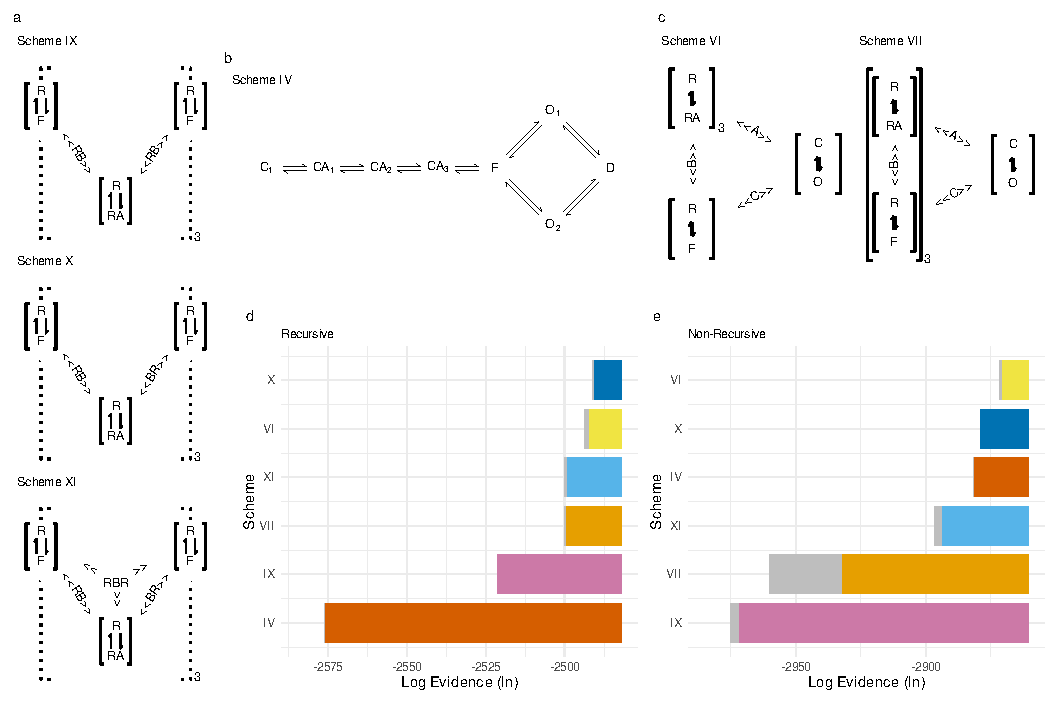
\includegraphics[width=\linewidth]{Figure_1.pdf}
	\caption{\textbf{Bayesian Evidence for Conformational, Allosteric, and Regular Models.}  
		(\textbf{a}) Schematic representation of the newly proposed Conformational models. R: resting; F: flipped; RA: agonist-bound; RB, BR: rotation-binding and binding-rotation allosteric couplings, indicating interactions with the left or right subunit; RBR: rotation-binding-rotation ternary allosteric coupling. Dotted lines indicate sections that are repeated three times, as specified by the subscript. In Scheme~IX, RB is equal to BR, in Scheme~X they differ, and in Scheme~XI ternary coupling is also present.  
		(\textbf{b}) Regular Scheme~IV. C: closed state; CA$_n$: closed state with $n$ agonists bound; F: flipped state; O$_n$: $n$th alternative open state; D: a potentially desensitized closed state where unbinding is restricted.  
		(\textbf{c}) Allosteric Schemes~VI and VII. C: closed channel; O: open channel; A, B, C: allosteric couplings; subscripts indicate the number of repetitions.  
		(\textbf{d--e}) Bayesian evidence for each illustrated scheme, computed using the recursive MacroIR algorithm (\textbf{d}) and the non-recursive MacroINR algorithm (\textbf{e}). Color coding is used to facilitate scheme ranking comparisons. Gray rectangles indicate the standard error of the log-evidence.  
	}
	\label{fig:figure1}
\end{figure}

Figure~1 displays Bayesian evidence for two allosteric models and one regular model—selected based on prior fitting performance—along with three new conformational models motivated by structural insights from P2X4. In these new models, receptor activation is driven by ATP binding at intersubunit interfaces that couples to independent rotational movements of each subunit. Two distinct secondary couplings—one on the left and one on the right—are proposed to mediate allosteric signaling, with channel conductance modeled as a function of the number of rotated subunits (maximal when all three are engaged).
\begin{comment}
The three newly introduced models aim to reflect the actual conformational changes observed in the crystal structures of the homologous P2X4 receptor. In particular, comparison of the closed and open structures of P2X4 suggests that channel activation involves a rotational movement of individual subunits. We hypothesize that, rather than occurring synchronously, this rotation can proceed independently in each of the three subunits. Moreover, the rotation is proposed to be allosterically coupled to ATP binding.

Since ATP binds at inter-subunit interfaces, our model accounts for two distinct allosteric couplings: (i) between ATP and the subunit to its left and (ii) between ATP and the subunit to its right. Each subunit, in turn, is subject to both types of interactions due to its two neighboring ATP binding sites. This reciprocal arrangement propagates allosteric interactions throughout the entire receptor complex.
\end{comment}


Within this framework, we derived four variants: Scheme~X incorporates distinct left and right couplings; Scheme~IX employs symmetric couplings; Scheme~VIII (Extended Data Fig.~1) features a ternary coupling mechanism (involving left rotation, binding, and right rotation); and Scheme~XI combines both independent and ternary interactions. In the ternary coupling paradigm, the presence of any two of the three conformational changes is required before the third is modulated, favoring a concerted opening mechanism.

In parallel, we evaluated Scheme~IV, a regular model derived by incorporating an intermediate flip state into a previously preferred single-channel scheme. This model comprises closed states with 0--4 bound ATP molecules, followed by a flip state that bifurcates into two open states, which subsequently converge into a final closed state—thus capturing the dynamics of receptor activation and deactivation. Two allosteric models, Schemes~VI and~VII, extend this framework by coupling three conformational transitions—binding, flipping, and gating—via all pairwise interactions. The sole difference between them is that Scheme~VI assumes concerted flipping across the entire channel, whereas Scheme~VII permits subunit-specific flipping.

Model performance was assessed using two likelihood approximations: MacroIR, a statistically robust recursive macroscopic interval integration method that accounts for temporal correlations, and MacroINR, a non-recursive variant that does not. Our results indicate that the non-recursive approximation yields a different evidence ranking, underscoring its inadequacy.

Among the tested models, Scheme~X—featuring independent left and right couplings without ternary interactions—achieved the highest Bayesian evidence, with Scheme~VI (synchronous flipping) following closely. A pronounced evidence gap between Scheme~X and Schemes~IX and~XI highlights significant asymmetry, with the data favoring independent secondary couplings over ternary interactions. Notably, the evidence for Scheme~VII, which comprises an expanded state space of approximately 40 states (compared to 24 or fewer in other schemes), could not be reliably estimated using MacroIR within the available computational time, and the regular Scheme~IV exhibited markedly lower evidence under the recursive method despite appearing more favorable under the non-recursive analysis.

Extended Data Figure~1 presents an analysis of five additional schemes: three Regular models (Schemes~I, II, and III), one Allosteric model (Scheme~V), and one new Conformational model (Scheme~VIII). Evidence comparisons reveal that incorporating a flip state substantially enhances model performance (Scheme~II vs I; IV vs III and VI and VII vs V) and that complex kinetic schemes outperform simpler models featuring a single open state (Scheme~IV vs II and III vs I). Moreover, a model relying solely on ternary coupling (Scheme~VIII) underperforms relative to Schemes~X and XI.

Collectively, these findings support a four-part hypothesis: (i) individual subunit rotation is feasible; (ii) ATP binding is allosterically coupled to the rotation of both the left and right subunits; (iii) these couplings differ in magnitude; and (iv) channel conductance is a function of the number of rotated subunits. This framework adequately accounts for the activation kinetics of P2X2 without invoking an additional, difficult-to-justify allosteric coupling between binding and gating, thereby reinforcing the validity of conformational models. We further interpret the flip state as the kinetic manifestation of individual subunit rotation.


\section{Analysis of the Posterior Distribution of Scheme X Parameters}
\begin{comment}
	Schemes cannot mathematically differentiate between interaction with the left subunit or the right subunit, there is no left-right information in the macrocurrents. Therefore it is not surprising that the posterior distribution of the allosteric parameters of Scheme X are all bimodal. As a way to break such symmetry in the priors we arbitrarily set BR to be 10 times RB. However, as the prior standard deviation of the $log10$ of both parameters (and all the remaining ones) was set to be 2, there was enough exploration at low thermodynamic temperatures to jump from one minimum to the other, so both values appear, although at different frequencies. 
	This bimodality can be removed by determining which is greater if RB or BR, and if the former if the case, swap all the remaining parameters. In this was unimodal distribution were recovered for all allosteric parameters. 
	Once we correct for the bimodality we find that whereas one interaction is considerable (100-10$^4$ times), the other is much smaller(0-2 times). So, upon binding, there is a strong allosteric interaction with one subunit and a weak interaction with the other. This second subunit will have strong interaction at the other binding site that it is forming. 
	If we then look at the decomposition of the allosteric interaction we see the following.
	
	
\end{comment}


The posterior distributions of parameters in Kinetic Scheme X (Fig.~X) reveal three distinct behavioral patterns. First, parameters governing kinetic rates, conductance, noise, inactivation constants, and baseline currents exhibit narrow, unimodal posteriors, indicating robust identifiability and strong data constraints. Second, two parameters describing the relationship between conductance and the number of rotated subunits---namely, the current leakage of the closed channel and the current-rotation coupling---show limited but consistent divergence from their priors, suggesting that the data confine their values to specific ranges, that is there is no information in the data to put a lower limit in the leakeage current. 
Finally, the parameters related to binding-rotation coupling display bimodal distributions, as anticipated given that kinetic data alone cannot resolve the inherent left-right symmetry of the allosteric coupling. Although weakly informative priors were employed to favor one pathway, the affine ensemble Monte Carlo sampling recovered both modes in proportions consistent with the prior, reflecting this symmetry.

To address this multimodality, we segregated the posterior samples into two subpopulations based on the dominant pathway (BR~$>$~RB or RB~$>$~BR) and reparameterized the system in terms of the difference in coupling energies, \(\Delta G = G_{BR} - G_{RB}\). This transformation collapsed the bimodal distribution into a unimodal one, ensuring practical identifiability without compromising the model's predictive power. This approach underscores how mechanistic symmetries can manifest as multimodality in Bayesian inference, necessitating targeted post-sampling analyses to extract interpretable parameters.


\begin{figure}[t]
	\centering
	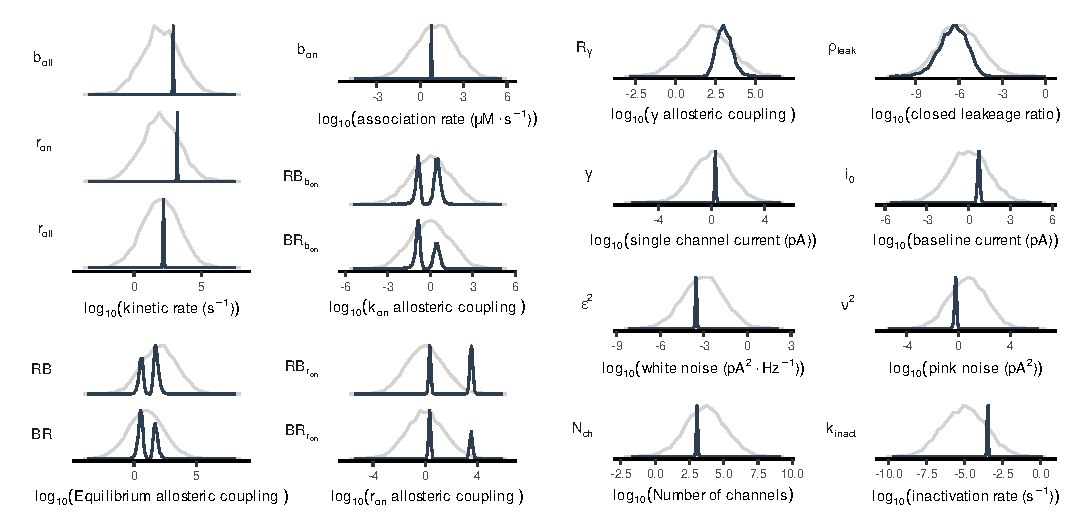
\includegraphics[width=\linewidth]{Figure_2.pdf}
	\caption{\textbf{Posterior distributions of model parameters for Scheme X.}  
		(\textbf{a}) Kinetic rate constants: \(r_{\text{on}}\) (rotation), \(r_{\text{off}}\) (return to resting state), and \(b_{\text{off}}\) (unbinding).  
		(\textbf{b}) Association rate: \(b_{\text{on}}\) (binding).  
		(\textbf{c}) Rotation-conductance coupling factor (\(R\gamma\)).  
		(\textbf{d}) Closed-channel leakage ratio (\(\rho_{\text{leak}}\)).  
		(\textbf{e}) Allosteric coupling factor affecting the binding rate (\(BR_{b_{\text{on}}}, RB_{b_{\text{on}}}\)).  
		(\textbf{f}) Single-channel current of the fully rotated channel (\(\gamma\)).  
		(\textbf{g}) Baseline current (\(i_0\)).  
		(\textbf{h}) White noise power (\(\epsilon^2\)).  
		(\textbf{i}) Pink noise power (\(\nu^2\)).  
		(\textbf{j}) Equilibrium allosteric coupling factors (\(BR, RB\)).  
		(\textbf{k}) Allosteric coupling factors affecting the rotation rate (\(BR_{r_{\text{on}}}, RB_{r_{\text{on}}}\)).  
		(\textbf{l}) Number of active channels (\(N_{\text{ch}}\)).  
		(\textbf{m}) Inactivation rate (\(k_{\text{inact}}\)).  
		The gray line represents the prior distribution, while the solid line indicates the posterior distribution. The probability density is normalized to its maximum value for each parameter.
	}
	\label{fig:posterior_SchemeX}
\end{figure}

\section{Structural Basis of Kinetic Rate Modulation}

Our kinetic schemes propose two distinct allosteric couplings, depending on whether modulation involves the subunit to the left or to the right of the ATP binding site. Figure~3a illustrates this concept, adapted from the original schematic that determined the open-channel structure of a purinergic receptor \cite{abierta_p2x}, where ATP binding is accompanied by the rotation of both ligand-contacting subunits. We extend that view by positing that subunits can rotate independently rather than synchronously, with ATP binding modulating these subtle conformational changes.

Traditional models of allosterism treat allosteric effects as modifications of equilibrium constants via a single coupling parameter. In contrast, our kinetic framework explicitly models the rate constants, thereby breaking the inherent symmetry—each conformational change (binding, rotation, gating, etc.) is governed by its own coupling parameter. This approach necessitates two additional parameters to fully describe the kinetic coupling.

Figure~3a depicts a cubic arrangement of three coupled conformational changes—agonist binding, left subunit rotation, and right subunit rotation. The vertices represent distinct state combinations (ranging from unrotated/free/unrotated to rotated/bound/rotated), and the edges are annotated with the kinetic expressions defining the transitions. In the absence of ATP, both subunits rotate at identical rates; however, ATP binding breaks this symmetry. (Note that this schematic is simplified, as it does not account for the influence of additional binding sites, which would require further allosteric factors.)

Figures~3b and 3c show representative posterior distributions for the kinetic rate constants associated with transitions involving a single subunit (i.e. \texttt{b\_on} versus \texttt{b\_off}). In Figure~3b, binding constants segregate into four clusters corresponding to distinct structural states: both subunits resting, left rotated, right rotated, and both rotated. Similarly, the rotation rate constants group according to binding site occupancy (both free, left occupied, right occupied, or both occupied). Colored lines in these plots indicate the magnitude of the allosteric coupling factors for both \textit{on} and \textit{off} transitions, while the diagonal axes represent log affinity [$\log(b_{\text{off}})-\log(b_{\text{on}})$] or log efficacy [$\log(r_{\text{on}})-\log(r_{\text{off}})$].

A clear asymmetry emerges between the left and right couplings. Specifically, the coupling associated with the right subunit (or equivalently, the binding site on the left) is strong, whereas that for the left subunit is weak. Moreover, an asymmetry is observed between binding and rotation: the binding data exhibit a well-separated cluster for the weak coupling, whereas the separation is less pronounced in the rotation rates. Notably, rotation of the left subunit markedly reduces the binding rate (\texttt{b\_on}, i.e. $RB_{b_{\text{on}}} \ll 1$), whereas rotation of the right subunit accelerates it ($BR_{b_{\text{on}}} > 1$).

Figure~3d further elucidates the kinetic allosteric coupling by plotting the logarithm of the \textit{on} rate coupling against that of the \textit{off} rate. A positive \textit{on} log factor indicates that the active state of the allosteric partner accelerates the transition, while a negative value denotes deceleration. Since the equilibrium constant is the ratio of the \textit{on} and \textit{off} rates, the overall allosteric effect is determined by the difference between these kinetic contributions. For example, if the mechanism solely stabilized the active state, one would expect a highly positive \textit{on} factor and a moderately negative \textit{off} factor; if it destabilized the resting state, the reverse would be true. When both mechanisms operate, the \textit{on} and \textit{off} factors should be of similar magnitude but opposite in sign—a pattern observed for $BR_{b_{\text{on}}}$, which appears to stabilize the bound state while only modestly destabilizing the free state.

Interestingly, two kinetic couplings deviate from these expectations. In one case, ATP binding at the left site increases both the \textit{on} and \textit{off} rates, suggesting a catalytic effect that lowers the energetic barrier for rotation while stabilizing the rotated state. Conversely, rotation of the left subunit reduces both binding and unbinding rates, yielding only a minor change in equilibrium but a substantial reduction in the \texttt{b\_on} rate. This observation implies an altered energetic barrier, possibly due to steric hindrance of the binding site upon rotation. By assuming a preexponential factor of $10^{-6}$, we calculated the posterior distributions of the corresponding energetic barriers, which illustrate the deduced changes in energy.


\section{From subunit behavior to collective behavior}
Previous analysis was focused on how kinetic coupling affect the kinetic rates of single subunits or binding sites. Figure 4 shows how to extend this behavior to the whole channel. In this squema, each subunit is represented by big ellipse, binding sites by a smaller one. Activated state (rotated or bound) is indicated as a filled elipse and resting states (no rotated or free) by an empty ellipse. The color coding of the arrows and ellipse indicates the interaction state for the underlying transition, grey indicating no interaction, orange the intense BR interaction, light blue the moderate RB and purple (sum of orange and ligth blue) the combination of both.  Vertical lines indicate rotations and horizontal lines indicate bindings/unbindings. As there are three subunits (binding sites) there are at most three vertical (horizontal ) arrows saliendo de cada estado. Cuando hay menos, por ejemplo del estado de inferior izquierdo, cada flecha puede indicar transiciones multiples, por lo que el kinetic rate se debe multiplicar por el numero de subunidades con el mismo estado de interaccion o color. 
Para saber cual es el kinetic rate de cualquier transicion se busca el estado de interaccion y con esa informacion se va a la figura 3, ahi se multiplica la tasa obtenida por numero de subunidades/sitio de union que  mismo estado de interaccion 
inicial. 

Con esta información se puede obtener la ocupancia de cada estado durante el experimento. Antes de cada pulso, se esperó 60 segundos desde la ultima aplicacion de ATP, porque solo los estados con 0 ATP unido tenian alguna ocupancia. Interesantemente (figura 5a), alrededor de un 15\% de los canales tenian una subunidad rotada, un 1\% dos y alrededor de 0.02\% tres subunidades rotadas. Fijense que a pesar de que no hay estimulo se observan fluctuaciones en la ocupancia. Esto se debe a que el algoritmo MacroIR atribuye las fluctuaciones estocásticas en la corriente a cambios en la proporcion de estados. 
En la figura 6b se observan la evolucion de una sample de la  posterior state probability desde que se comienza la aplicación del pulso. Notar la escala logarimica. Se comienza en el estado libre de ATP y en descanso y se van llenando los sitios de unión y luego rotando las subunidades. Interesantemente, en la activación a alta concentracion de ATP, el camino principal  es por los bordes del esquema, mientras que la desactivación hay una significativa contribución de los estados centrales, es decir parcialmente ligados y parcialmente rotados. 
En la figura 4C se grafica la distribucion a posteriori de la corriente para 0,1,2 y 3 subunidades rotadas. Mientras que la corriente asignada a 0 y 1 subunidad rotada es insignificante, es notable que haya una corriente mas baja pero significativa con dos subunidades rotadas. Si observamos la proporcion de canales con tres y dos subunidades rotadas en ausencia de ligando vemos que la corriente sin ligando es mayoritariamente debida a la conductancia de dos subunidades rotadas. 

Se ha observado consistentemente en la literatura que dos sitios de union al ATP funcionales alcanzan para generar una respuesta. Este grafico explica porqué. 


\section{De los estados a la likelihood y mas allá}
Con la información de la probabilidad de los estados y la conductancia se puede calcular la corriente esperada (figura 6 a). Vemos que existen fluctuaciones en la corriente pre-pulso que MacroIR puede reproducir. Reproduce con trampa, ya que usa la información de la medida anterior para predecir la próxima, pero obtiene información cinética (y como vimos en la figura anterior, de conductancia) en el camino. Como se ve en la figura, el esquema 10 reproduce el perfil temporal de la respuesta de forma excelente. 
Ahora, excelente no es un concepto cientifico, necesitamos algo mejor, una likelihood. Para obtener una likelihood necesitamos una varianza y eso también lo entrega MacoIR. La varianza tiene tres componentes, el ruido estocástico generado por los cambios aleatorios de los estados, el ruido instrumental blanco (que disminuye con la duración de los intervalos de promediación) y un ruido rosa que modela otros procesos estocásticos no reproducidos por el esquema 10. Estos procesos pueden ser otros canales o detalles de la cinética que no son tomados por el esquema 10. Como se ve en la figura el ruido rosa es reducido, pero su distribución a posteriori es acotada, de modo que algo contribuye. El ruido blanco es significativo para las mediciones mas breves a concentracion baja de ATP, mientras que el ruido estocástico es mayoritario en el resto de los casos. Esto implica que hay mucha información disponible en estas fluctuaciones estocasticas, explicando la deficiencia de MacroINR para reproducir el ranking de modelos cineticos. 

Finalmente con la varianza y la corriente esperada podemos calcular la likelihood de cada medicion, es decir una medida precisa de qué tan bueno es el modelo para predecir los datos. También se puede calcular la esperanza de la likelihood y compararla con la likelihood obtenida. Un modelo deficiente, que no modele bien la distribución y correlación de los errores mostraría una gran divergencia entre la likelihood esperada y la observada y como se ve en la figura este no es el caso. Salvo algunos outliers, la mayoria de las observaciones tienen una likeilihood cercana a la esperada. 

\section{Discussion}

\subsection*{Integrating structure and kinetics}
The dynamic behavior of ion channels has long been interpreted through equilibrium-driven allosteric models or phenomenological kinetic schemes divorced from structural insights. Here, we resolve this divide by introducing a conformational kinetic framework that directly links discrete structural transitions to experimentally observed macro-currents. Our findings not only validate the predictive power of kinetic-conformational modeling but also redefine principles of allosteric regulation, emphasizing kinetic coupling as a critical evolutionary driver. 

Central to our approach is the \textit{conformational model}, which posits that kinetic rate constants ($k_{\text{on}}$, $k_{\text{off}}$) and their couplings correspond to precise structural rearrangements (e.g., domain rotations). This contrasts with classical allostery, where ligand-binding equilibria dominate interpretations. As shown in Fig.~\ref{fig:model}, inhibitory couplings observed in our two-effector system suggest conformational transitions are actively suppressed unless specific energetic thresholds are met—a mechanism we term \textit{kinetic gating}.

\subsection*{Evolutionary optimization through kinetic coupling}
\begin{itemize}
	\item Reduced transition frequencies: Data clustering in inhibitory quadrants (Fig.~\ref{fig:quadrants}) implies evolutionary selection against high-frequency conformational changes. 
	\item Kinetic stability: Modulating energy barriers (e.g., $\Delta G^{\ddagger}_{\text{rot}}$) minimizes exposure of vulnerable residues to oxidative damage while preserving functional flexibility.
\end{itemize}

\subsection*{Beyond classical allostery}
Our framework extends allostery to non-equilibrium regimes. Traditional models (Eq.~1):

\begin{equation}
	K_{\text{eq}} = \frac{[C_{\text{open}}]}{[C_{\text{closed}}]}
\end{equation}

neglect transition-state regulation. In contrast, kinetic coupling (Eq.~2):

\begin{equation}
	\kappa = \frac{k_{\text{cat}}^{\text{effector\ bound}}}{k_{\text{cat}}^{\text{apo}}}
\end{equation}

reveals how evolution optimizes \textit{transition paths} rather than just equilibrium states. Lowering rotational barriers (Fig.~\ref{fig:barriers}) implements "kinetic proofreading" against spurious activation.

\subsection*{Limitations and future directions}
\begin{enumerate}
	\item Scalability to multimeric systems
	\item Continuous vs. discrete conformational states
	\item Role of lipid interactions (see Supplementary Fig.~7)
\end{enumerate}

\subsection*{Broader implications}
\begin{itemize}
	\item Precision pharmacology: Targeting kinetic couplings ($\kappa$) over binding affinities ($K_d$)
	\item Oxidative resilience: Engineered proteins with optimized $\Delta G^{\ddagger}$ landscapes
\end{itemize}

\paragraph*{Conclusion} We establish kinetic coupling as a fundamental mechanism balancing functional dynamics with structural resilience. This paradigm shift—from equilibrium to kinetic control—reconciles discrepancies between structural and functional studies while opening new avenues for understanding allostery and disease 


\section{Discussion}\label{discussion}
\subsection{Mechanistic Significance of Scheme 10}
The mechanistic insights from Scheme 10 suggest that global channel behavior can emerge from local conformational changes and their interactions. This aligns with structural studies proposing that subunit rotation is a key gating determinant in ligand-gated ion channels.

The novel modeling of current as a function of rotated subunits offers two interpretations:
\begin{enumerate}
    \item \textbf{Ultrafast Gating:} The gating process is faster than the experiment’s resolution, resulting in an average current.
    \item \textbf{Dynamic Pore Size:} The pore’s conductance might increase with the number of rotated subunits.
\end{enumerate}

These interpretations provide a mechanistic link between observed macroscopic currents and hypothesized structural transitions.

\subsection{Comparison to Conventional Models}
Although Scheme 4 achieved the highest evidence, its complex state transitions (e.g., flip states and disconnected closed states) remain challenging to correlate with structural changes. In contrast, Scheme 10 offers a parsimonious explanation with clear mechanistic relevance.

\subsection{Broader Implications}
The ability to test hypotheses of symmetric vs. asymmetric coupling and synchronous vs. sequential subunit rotation highlights the value of Bayesian evidence for model comparison. These findings suggest that asymmetric and sequential mechanisms are likely key features of P2X2 activation.

\newpage




\begin{comment}

    
\section{Tables}\label{sec5}


\begin{table}[h]
\caption{Posterior distribution of Scheme X}\label{tab1}%
\begin{tabular}{c|c|c|c}
\hline
\hline
  parameters & median & CI\_hdi\_low & CI\_hdi\_hi \\ 
\hline
\hline
  \rowcolor[HTML]{efefef} 
  RB & 632.661 & 0.1441125 & 3.918861 10^{3} \\ 
  RB_{rot} & 2.454486 10^{4} & 1.260341 & 1.401152 10^{5} \\ 
  \rowcolor[HTML]{efefef} 
  RB_{bon} & 6.248909 & 1.933688 10^{-6} & 38.56124 \\ 
  BR & 1.612385 & 0.2657464 & 1.106451 10^{3} \\ 
  \rowcolor[HTML]{efefef} 
  BR_{rot} & 2.241492 & 1.077178 & 3.979711 10^{4} \\ 
  BR_{bon} & 6.986098 10^{-3} & 9.626552 10^{-7} & 11.16657 \\ 
\hline
\hline
\end{tabular}
\footnotetext{Source: This is an example of table footnote. This is an example of table footnote.}
\footnotetext[1]{Example for a first table footnote. This is an example of table footnote.}
\footnotetext[2]{Example for a second table footnote. This is an example of table footnote.}
\end{table}




\noindent

The input format for the above table is as follows:




\begin{table}[h]
\caption{Example of a lengthy table which is set to full textwidth}\label{tab2}
\begin{tabular*}{\textwidth}{@{\extracolsep\fill}lcccccc}
\toprule%
& \multicolumn{3}{@{}c@{}}{Element 1\footnotemark[1]} & \multicolumn{3}{@{}c@{}}{Element 2\footnotemark[2]} \\\cmidrule{2-4}\cmidrule{5-7}%
Project & Energy & $\sigma_{calc}$ & $\sigma_{expt}$ & Energy & $\sigma_{calc}$ & $\sigma_{expt}$ \\
\midrule
Element 3  & 990 A & 1168 & $1547\pm12$ & 780 A & 1166 & $1239\pm100$\\
Element 4  & 500 A & 961  & $922\pm10$  & 900 A & 1268 & $1092\pm40$\\
\botrule
\end{tabular*}
\footnotetext{Note: This is an example of table footnote. This is an example of table footnote this is an example of table footnote this is an example of~table footnote this is an example of table footnote.}
\footnotetext[1]{Example for a first table footnote.}
\footnotetext[2]{Example for a second table footnote.}
\end{table}

In case of double column layout, tables which do not fit in single column width should be set to full text width. For this, you need to use \verb+\begin{table*}+ \verb+...+ \verb+\end{table*}+ instead of \verb+\begin{table}+ \verb+...+ \verb+\end{table}+ environment. Lengthy tables which do not fit in textwidth should be set as rotated table. For this, you need to use \verb+\begin{sidewaystable}+ \verb+...+ \verb+\end{sidewaystable}+ instead of \verb+\begin{table*}+ \verb+...+ \verb+\end{table*}+ environment. This environment puts tables rotated to single column width. For tables rotated to double column width, use \verb+\begin{sidewaystable*}+ \verb+...+ \verb+\end{sidewaystable*}+.

\begin{sidewaystable}
\caption{Tables which are too long to fit, should be written using the ``sidewaystable'' environment as shown here}\label{tab3}
\begin{tabular*}{\textheight}{@{\extracolsep\fill}lcccccc}
\toprule%
& \multicolumn{3}{@{}c@{}}{Element 1\footnotemark[1]}& \multicolumn{3}{@{}c@{}}{Element\footnotemark[2]} \\\cmidrule{2-4}\cmidrule{5-7}%
Projectile & Energy	& $\sigma_{calc}$ & $\sigma_{expt}$ & Energy & $\sigma_{calc}$ & $\sigma_{expt}$ \\
\midrule
Element 3 & 990 A & 1168 & $1547\pm12$ & 780 A & 1166 & $1239\pm100$ \\
Element 4 & 500 A & 961  & $922\pm10$  & 900 A & 1268 & $1092\pm40$ \\
Element 5 & 990 A & 1168 & $1547\pm12$ & 780 A & 1166 & $1239\pm100$ \\
Element 6 & 500 A & 961  & $922\pm10$  & 900 A & 1268 & $1092\pm40$ \\
\botrule
\end{tabular*}
\footnotetext{Note: This is an example of table footnote this is an example of table footnote this is an example of table footnote this is an example of~table footnote this is an example of table footnote.}
\footnotetext[1]{This is an example of table footnote.}
\end{sidewaystable}

\section{Figures}\label{sec6}

As per the \LaTeX\ standards you need to use eps images for \LaTeX\ compilation and \verb+pdf/jpg/png+ images for \verb+PDFLaTeX+ compilation. This is one of the major difference between \LaTeX\ and \verb+PDFLaTeX+. Each image should be from a single input .eps/vector image file. Avoid using subfigures. The command for inserting images for \LaTeX\ and \verb+PDFLaTeX+ can be generalized. The package used to insert images in \verb+LaTeX/PDFLaTeX+ is the graphicx package. Figures can be inserted via the normal figure environment as shown in the below example:

%%=============================================%%
%% For presentation purpose, we have included  %%
%% \bigskip command. Please ignore this.       %%
%%=============================================%%
\bigskip
\begin{verbatim}
\begin{figure}[<placement-specifier>]
\centering
\includegraphics{<eps-file>}
\caption{<figure-caption>}\label{<figure-label>}
\end{figure}
\end{verbatim}
\bigskip
%%=============================================%%
%% For presentation purpose, we have included  %%
%% \bigskip command. Please ignore this.       %%
%%=============================================%%


\begin{figure}[h]
\centering
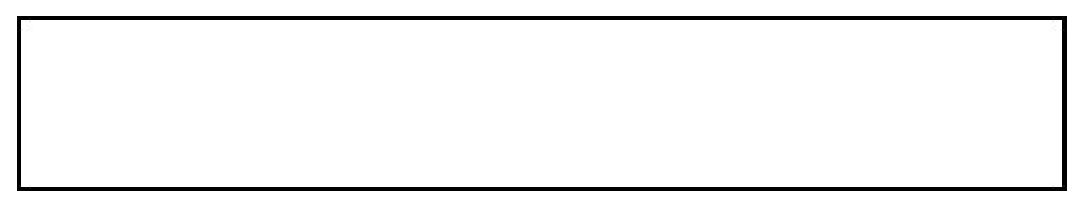
\includegraphics[width=0.9\textwidth]{fig.eps}
\caption{This is a widefig. This is an example of long caption this is an example of long caption  this is an example of long caption this is an example of long caption}\label{fig1}
\end{figure}

In case of double column layout, the above format puts figure captions/images to single column width. To get spanned images, we need to provide \verb+\begin{figure*}+ \verb+...+ \verb+\end{figure*}+.

For sample purpose, we have included the width of images in the optional argument of \verb+\includegraphics+ tag. Please ignore this. 

\section{Algorithms, Program codes and Listings}\label{sec7}

Packages \verb+algorithm+, \verb+algorithmicx+ and \verb+algpseudocode+ are used for setting algorithms in \LaTeX\ using the format:

%%=============================================%%
%% For presentation purpose, we have included  %%
%% \bigskip command. Please ignore this.       %%
%%=============================================%%
\bigskip
\begin{verbatim}
\begin{algorithm}
\caption{<alg-caption>}\label{<alg-label>}
\begin{algorithmic}[1]
. . .
\end{algorithmic}
\end{algorithm}
\end{verbatim}
\bigskip
%%=============================================%%
%% For presentation purpose, we have included  %%
%% \bigskip command. Please ignore this.       %%
%%=============================================%%

You may refer above listed package documentations for more details before setting \verb+algorithm+ environment. For program codes, the ``verbatim'' package is required and the command to be used is \verb+\begin{verbatim}+ \verb+...+ \verb+\end{verbatim}+. 

Similarly, for \verb+listings+, use the \verb+listings+ package. \verb+\begin{lstlisting}+ \verb+...+ \verb+\end{lstlisting}+ is used to set environments similar to \verb+verbatim+ environment. Refer to the \verb+lstlisting+ package documentation for more details.

A fast exponentiation procedure:

\lstset{texcl=true,basicstyle=\small\sf,commentstyle=\small\rm,mathescape=true,escapeinside={(*}{*)}}
\begin{lstlisting}
begin
  for $i:=1$ to $10$ step $1$ do
      expt($2,i$);  
      newline() od                (*\textrm{Comments will be set flush to the right margin}*)
where
proc expt($x,n$) $\equiv$
  $z:=1$;
  do if $n=0$ then exit fi;
     do if odd($n$) then exit fi;                 
        comment: (*\textrm{This is a comment statement;}*)
        $n:=n/2$; $x:=x*x$ od;
     { $n>0$ };
     $n:=n-1$; $z:=z*x$ od;
  print($z$). 
end
\end{lstlisting}

\begin{algorithm}
\caption{Calculate $y = x^n$}\label{algo1}
\begin{algorithmic}[1]
\Require $n \geq 0 \vee x \neq 0$
\Ensure $y = x^n$ 
\State $y \Leftarrow 1$
\If{$n < 0$}\label{algln2}
        \State $X \Leftarrow 1 / x$
        \State $N \Leftarrow -n$
\Else
        \State $X \Leftarrow x$
        \State $N \Leftarrow n$
\EndIf
\While{$N \neq 0$}
        \If{$N$ is even}
            \State $X \Leftarrow X \times X$
            \State $N \Leftarrow N / 2$
        \Else[$N$ is odd]
            \State $y \Leftarrow y \times X$
            \State $N \Leftarrow N - 1$
        \EndIf
\EndWhile
\end{algorithmic}
\end{algorithm}

%%=============================================%%
%% For presentation purpose, we have included  %%
%% \bigskip command. Please ignore this.       %%
%%=============================================%%
\bigskip
\begin{minipage}{\hsize}%
\lstset{frame=single,framexleftmargin=-1pt,framexrightmargin=-17pt,framesep=12pt,linewidth=0.98\textwidth,language=pascal}% Set your language (you can change the language for each code-block optionally)
%%% Start your code-block
\begin{lstlisting}
for i:=maxint to 0 do
begin
{ do nothing }
end;
Write('Case insensitive ');
Write('Pascal keywords.');
\end{lstlisting}
\end{minipage}

\end{comment}

\section{Discussion}
\label{dis}


\section{Conclusion}
\label{con}


\backmatter

\bmhead{Supplementary information}

If your article has accompanying supplementary file/s please state so here. 

Authors reporting data from electrophoretic gels and blots should supply the full unprocessed scans for key as part of their Supplementary information. This may be requested by the editorial team/s if it is missing.

Please refer to Journal-level guidance for any specific requirements.

\bmhead{Acknowledgements}


Acknowledgements are not compulsory. Where included they should be brief. Grant or contribution numbers may be acknowledged.

Please refer to Journal-level guidance for any specific requirements.

\section*{Declarations}

Some journals require declarations to be submitted in a standardised format. Please check the Instructions for Authors of the journal to which you are submitting to see if you need to complete this section. If yes, your manuscript must contain the following sections under the heading `Declarations':

\begin{itemize}
\item Funding
\item Conflict of interest/Competing interests (check journal-specific guidelines for which heading to use)
\item Ethics approval and consent to participate
\item Consent for publication
\item Data availability 
\item Materials availability
\item Code availability 
\item Author contribution
\end{itemize}

\noindent
If any of the sections are not relevant to your manuscript, please include the heading and write `Not applicable' for that section. 

%%===================================================%%
%% For presentation purpose, we have included        %%
%% \bigskip command. Please ignore this.             %%
%%===================================================%%
\bigskip
\begin{flushleft}%
Editorial Policies for:

\bigskip\noindent
Springer journals and proceedings: \url{https://www.springer.com/gp/editorial-policies}

\bigskip\noindent
Nature Portfolio journals: \url{https://www.nature.com/nature-research/editorial-policies}

\bigskip\noindent
\textit{Scientific Reports}: \url{https://www.nature.com/srep/journal-policies/editorial-policies}

\bigskip\noindent
BMC journals: \url{https://www.biomedcentral.com/getpublished/editorial-policies}
\end{flushleft}

\begin{appendices}

\section{Section title of first appendix}\label{secA1}
\section{Supplementary Material}

\subsection{Detailed Kinetic Schemes}
Figure S1 and Table S1 provide detailed descriptions of all 11 kinetic schemes, including their state diagrams, parameterizations, and mechanistic assumptions.

\subsection{Bayesian Evidence and Posterior Distributions}
Figures S2-S5 present the Bayesian evidence and posterior distributions for all models, allowing readers to evaluate their relative plausibility.

\subsection{Equations for Current Modeling}
The derivation of the current equation \( i(n) = i_{\text{max}} \cdot \frac{E_n}{E_n + 1} \) and its implications for state-space reduction are detailed in Section S2.

\subsection{Alternative Hypotheses}
Comparative evidence for symmetric coupling (Scheme 9), ternary interactions (Scheme XI), and synchronous rotation (Scheme VI) are discussed in Section S3, providing a deeper understanding of their limitations.

\begin{equation}
    r^{on}_{.BR}= r^{on} \cdot RBR^{on}_{.BR} 
	\label{eq:ron_BR}
\end{equation}
\begin{equation}
    r^{on}_{R.R}= r^{on} \cdot RBR^{on}_{R.R} 
	\label{eq:ronR_R}
\end{equation}
\begin{equation}
    r^{on}_{RB.}= r^{on} \cdot RBR^{on}_{RB.} 
	\label{eq:ronRB_}
\end{equation}
las constantes reversas se obtienen 
\begin{equation}
    r^{off}_{.BR}= r^{off} \cdot RBR^{off}_{.BR} 
	\label{eq:roff_BR}
\end{equation}
\begin{equation}
    RBR^{off}_{.BR} = \frac{RBR^{on}_{.BR}}{RBR}  \label{eq:RBRoff_BR}
\end{equation}




An appendix contains supplementary information that is not an essential part of the text itself but which may be helpful in providing a more comprehensive understanding of the research problem or it is information that is too cumbersome to be included in the body of the paper.

%%=============================================%%
%% For submissions to Nature Portfolio Journals %%
%% please use the heading ``Extended Data''.   %%
%%=============================================%%

%%=============================================================%%
%% Sample for another appendix section			       %%
%%=============================================================%%

%% \section{Example of another appendix section}\label{secA2}%
%% Appendices may be used for helpful, supporting or essential material that would otherwise 
%% clutter, break up or be distracting to the text. Appendices can consist of sections, figures, 
%% tables and equations etc.

\end{appendices}

%%===========================================================================================%%
%% If you are submitting to one of the Nature Portfolio journals, using the eJP submission   %%
%% system, please include the references within the manuscript file itself. You may do this  %%
%% by copying the reference list from your .bbl file, paste it into the main manuscript .tex %%
%% file, and delete the associated \verb+\bibliography+ commands.                            %%
%%===========================================================================================%%

\bibliography{biblio}% common bib file
%% if required, the content of .bbl file can be included here once bbl is generated
%%\input sn-article.bbl


\end{document}
